\documentclass[11pt]{amsart}

% Manuscript v8: consolidated exposition.

\usepackage{amsmath,amssymb,mathtools}
\usepackage{booktabs}
\usepackage{array}
\usepackage{enumitem}
\usepackage{xcolor}
\usepackage[protrusion=true,expansion=false]{microtype}
\usepackage{geometry}
\usepackage{graphicx}
\usepackage{placeins}
\graphicspath{{figures/}}
\usepackage{bm}
\usepackage{url}
\usepackage{textcomp}
\usepackage{hyperref}
\geometry{margin=1in}
\setlength{\emergencystretch}{1em}
\renewcommand{\topfraction}{0.95}
\renewcommand{\bottomfraction}{0.9}
\renewcommand{\textfraction}{0.05}
\renewcommand{\floatpagefraction}{0.65}
\hypersetup{hidelinks,
 pdftitle={Residual Certification of Neural and Reduced Surrogates for Tempered-Fractional CGMY Pricing PIDEs},
 pdfauthor={Davood Damircheli},
 pdfsubject={Discrete residual certification; manuscript v8},
 pdfkeywords={CGMY, residual certification, neural surrogate, POD, option pricing}}

\newtheorem{theorem}{Theorem}[section]
\newtheorem{proposition}[theorem]{Proposition}
\newtheorem{lemma}[theorem]{Lemma}
\newtheorem{corollary}[theorem]{Corollary}
\newtheorem{assumption}[theorem]{Assumption}
\newtheorem{definition}[theorem]{Definition}
\theoremstyle{remark}
\newtheorem{remark}[theorem]{Remark}

% ---------------------- provenance callouts -----------------------

% ----------------------------- notation --------------------------
\newcommand{\R}{\mathbb{R}}
\newcommand{\Pset}{\mathcal{P}}
\newcommand{\Sop}{\mathcal{S}}
\newcommand{\Vh}{V_h^0}
\newcommand{\Vmu}{V_{\mu}}
\newcommand{\Vp}[1]{V_{#1}}
\newcommand{\Mh}{M_h}
\newcommand{\Ah}{A_h}
\newcommand{\Sh}{S_h}
\newcommand{\norm}[1]{\left\lVert #1\right\rVert}
\newcommand{\ip}[2]{\left\langle #1,#2\right\rangle}
\newcommand{\dt}{\Delta\tau}
\newcommand{\etaSharp}{\eta_{\mathrm{sh}}}
\newcommand{\etaMass}{\eta_{\mathrm{ms}}}
\newcommand{\etaGuar}{\eta_{\mathrm{gu}}}
\newcommand{\ee}{\mathbf e}
\newcommand{\cc}{\mathbf c}
\newcommand{\rr}{\bm\rho}
\newcommand{\ff}{\mathbf f}
\newcommand{\vv}{\mathbf v}
\newcommand{\bb}{\mathbf b}
\newcommand{\zz}{\mathbf z}
\newcommand{\yy}{\mathbf y}
\newcommand{\ww}{\mathbf w}
\newcommand{\sres}{\mathbf s}
\newcommand{\dd}{\bm\delta}
\newcommand{\rf}{r}
\newcommand{\Hs}{H^{s_\mu}_{M,G}}
\newcommand{\Dm}{\mathcal D_G^-}
\newcommand{\Dp}{\mathcal D_M^+}
\newcommand{\Aop}{\mathcal A_\mu}
\DeclareMathOperator{\Real}{Re}

\title[Residual Certification for CGMY Pricing Trajectories]
      {Residual Certification of Neural and Reduced Surrogates for\\ Tempered-Fractional CGMY Pricing PIDEs}
\author{Davood Damircheli}
\address{Department of Mathematics, Louisiana State University,
Baton Rouge, LA 70803, USA}
\date{}

\subjclass[2020]{65M60, 65M15, 65T50, 68T07, 91G20, 60G51}
\keywords{CGMY process, neural operator, certified scientific machine
learning, B-spline Galerkin method, tempered fractional PIDE, a posteriori
error estimation, residual certification, operator learning, option pricing}

\begin{document}
\begin{abstract}
We develop residual error bounds for neural and reduced approximations of
European-put pricing trajectories under the Carr--Geman--Madan--Yor model.
A Crank--Nicolson energy estimate combines the initial discrepancy with an
accumulated dual residual norm in the constrained spline space. A two-sided
Riesz bracket supplies an upper bound even when iterative solves are
incomplete, enabling tolerance-controlled acceptance and correction.
The guarantees concern the assembled discrete problem in exact arithmetic;
the implementation is evaluated in ordinary floating point.
Matched benchmarks show that the neural workflow is slower than an
optimised direct solve, whereas a mass-weighted POD approximation achieves
direct acceptance and lower online cost. Assembly and certification dominate
the optimised solver costs. Independent Fourier prices and refinement
studies distinguish the certified surrogate error from spatial, temporal
and domain errors. The resulting framework provides scheme-consistent
certification and a quantitative account of its computational value.
\end{abstract}
\maketitle

\section{Introduction}
\label{sec:introduction}
The CGMY tempered-stable process models asymmetric jumps and small-jump
activity through four parameters \cite{CarrGemanMadanYor2002}. European
pricing under this model leads to a nonlocal, nonsymmetric parabolic PIDE
whose fractional order varies with the model parameters
\cite{CarteadelCastilloNegrete2007}. Repeated pricing, calibration and
uncertainty quantification motivate approximations of the parameter-to-price
map. An aggregate prediction error, however, provides no error bound for an
individual query outside well-represented regions of the training set.

Neural solution maps, including DeepONet \cite{LuJinPangZhangKarniadakis2021}
and Fourier neural operators \cite{LiKovachkiEtAl2021,KovachkiEtAl2023},
provide expressive surrogate models. Nonlocal kernel networks explicitly
incorporate nonlocal structure \cite{YouYuDEliaGaoSilling2022}, while neural
reduced models learn coordinates in a prescribed trial space
\cite{HesthavenUbbiali2018,BhattacharyaEtAl2021}. Query-wise residual bounds
originate in certified reduced-basis methods for parametric evolution
problems \cite{GreplPatera2005,RozzaHuynhPatera2008,HaasdonkOhlberger2008}
and option pricing \cite{ContLantosPironneau2011}. Variationally correct
operator learning emphasises that the residual norm must reflect stability
of the underlying problem \cite{QiuDahmenChen2026}.

This paper combines these ideas for CGMY pricing with a spline-valued
surrogate. The deterministic discretisation defines the coefficient space,
training trajectories, residual and correction operator. Established
finite-difference, Galerkin and transform methods supply the wider numerical
context \cite{ContVoltchkova2005,MatacheVonPetersdorffSchwab2004,
HilberReichmannSchwabWinter2013,FangOosterlee2008}; the spline construction
follows \cite{DamircheliCGMY2026}. The specific analytical features are the
parameter-dependent energy order, the nonsymmetric fractional operator,
and the restriction to free coefficients after imposing exterior data.

The contributions are:
\begin{enumerate}[leftmargin=2em]
\item parameter-uniform continuity and coercivity for an interior CGMY
family, with explicit constants;
\item a scheme-consistent discrete residual bound including the initial
error, and a two-sided bracket for incomplete Riesz solves;
\item tolerance-controlled prediction, boundary projection, certification
and correction using one constrained algebraic system;
\item matched evaluations of neural, POD and deterministic methods,
including certificate verification, timing, assembly and price refinement.
\end{enumerate}
The principal computational finding is that certification enables reliable
selection of candidate trajectories, but the tested neural approximation
requires correction at every benchmark query and offers no speed advantage
over an optimised direct solve. A sufficiently rich POD space passes the
same tolerance directly and reduces online cost.

The analysis distinguishes the assembled discrete system from the exact
Galerkin discretisation and the continuum price. Residual certification
controls distance to the exact solution of the first. The variational
results describe the second under exact assembly, and Fourier comparisons
assess the third empirically. The numerical implementation uses ordinary
floating point; its arithmetic assumptions are stated with the bracket.

Section~\ref{sec:model} defines the model and constrained discretisation.
Section~\ref{sec:operator} describes the candidate approximations.
Section~\ref{sec:certificate} develops certification and correction,
Section~\ref{sec:numerics} evaluates them, and
Section~\ref{sec:conclusion} interprets the findings.
Appendix~\ref{app:proofs} gives uniform-stability proofs and supporting
extensions. Throughout, $\psi$ denotes the payoff, $g$ its exterior lifting,
$\mu=(C,G,M,Y,r)$ the spatial-operator parameters, and $T$ the maturity.
\section{CGMY model and constrained discretisation}
\label{sec:model}\label{sec:galerkin}
\subsection{CGMY backward operator}
\label{ssec:operator}

Let $S_t=e^{X_t}$ under a risk-neutral measure and let $V(x,\tau)$ be the
option value in the log-price variable $x=\log S$ and backward time
$\tau=T-t$.  Following the convention of the companion paper
\cite{DamircheliCGMY2026}, the CGMY parameters satisfy
\begin{equation}
  C>0,\qquad G>0,\qquad M>1,\qquad Y\in(0,2),\qquad Y\ne1,
  \label{eq:cgmy-parameters}
\end{equation}
where $M>1$ is the exponential-moment condition that makes the stock
martingale correction
\begin{equation}
  \omega_S(\mu)
  = C\Gamma(-Y)\bigl[(M-1)^Y-M^Y+(G+1)^Y-G^Y\bigr]
  \label{eq:martingale-correction}
\end{equation}
real valued.  Set
\begin{equation}
  \lambda_0(\mu) := \rf + C\Gamma(-Y)\bigl(M^Y+G^Y\bigr).
  \label{eq:lambda0}
\end{equation}
For $Y\in(1,2)$ one has $\Gamma(-Y)>0$ and hence $\lambda_0>\rf$.  The
tempered left- and right-sided Riemann--Liouville operators are
\begin{equation}
  \Dm u=e^{-Gx}\,{}_{-\infty}D_x^Y\bigl(e^{Gx}u\bigr),
  \qquad
  \Dp u=e^{Mx}\,{}_{x}D_\infty^Y\bigl(e^{-Mx}u\bigr),
  \label{eq:tempered-ops}
\end{equation}
and the single backward-time operator used for both the theory and the
discretisation is
\begin{equation}
  \Aop u
  =-(\rf-\omega_S)u_x
   -C\Gamma(-Y)\Dp u
   -C\Gamma(-Y)\Dm u
   +\lambda_0u.
  \label{eq:cgmy-operator}
\end{equation}
The European pricing problem is
\begin{equation}
  \partial_\tau V+\Aop V=0,
  \qquad
  V(\cdot,0)=\psi.
  \label{eq:pricing-pide}
\end{equation}
On the full line the Fourier symbols are
$\widehat{\Dm u}(\xi)=(G+i\xi)^Y\widehat u(\xi)$ and
$\widehat{\Dp u}(\xi)=(M-i\xi)^Y\widehat u(\xi)$ on the principal branch, so
that
\begin{equation}
  A_\mu(\xi)
  =-(\rf-\omega_S)i\xi
   -C\Gamma(-Y)\bigl[(M-i\xi)^Y+(G+i\xi)^Y\bigr]
   +\lambda_0 .
  \label{eq:symbol}
\end{equation}

\subsection{Parameter family and exterior data}
\label{ssec:family}\label{ssec:finite-domain}
The coefficient parameters lie in the compact interior box
\begin{equation}
\begin{aligned}
 \Pset=\bigl\{\mu=(C,G,M,Y,\rf):\;&
 C\in[C_{\min},C_{\max}],\quad C_{\min}>0,\\
 &G\in[G_{\min},G_{\max}],\quad G_{\min}>0,\\
 &M\in[M_{\min},M_{\max}],\quad M_{\min}>1,\\
 &Y\in[Y_{\min},Y_{\max}]\Subset(1,2),\\
 &\rf\in[r_{\min},r_{\max}],\quad r_{\min}>0\bigr\}.
\end{aligned}
 \label{eq:parameter-set}
\end{equation}

Maturity $T$ is an additional surrogate input determining the time horizon;
$\psi$ is the payoff. The numerical parameter ranges are listed in
Table~\ref{tab:proposed-box}.
\begin{table}[ht]
\centering\small
\caption{Parameter family for the fixed-strike numerical study.}
\label{tab:proposed-box}
\begin{tabular}{lllllll}
\toprule
$C$ & $G$ & $M$ & $Y$ & $r$ & $T$ (years) & $K$\\
\midrule
$[0.05,1]$ & $[1,5]$ & $[2,9]$ & $[1.1,1.8]$ & $[0.01,0.1]$ & $[0.1,1]$ & $100$\\
\bottomrule
\end{tabular}
\end{table}
The restrictions $C_{\min}>0$, $r_{\min}>0$ and
$[Y_{\min},Y_{\max}]\Subset(1,2)$ give uniform coercivity.
The condition $M_{\min}>1$ selects the interior exponential-moment regime.
A common truncated domain $\Omega=(x_{\min},x_{\max})$ is used throughout
the family.

Nonlocal exterior values enter through $V=g+U$, with $U$ extended by zero
outside $\Omega$. For a put, a smooth lifting is
$g(x,\tau)=(Ke^{-r\tau}-e^x)\zeta(x)$, where $\zeta$ equals one to the left
of the domain and zero to its right. With $s_\mu=Y/2$, define
\begin{equation}
  \Vmu=\Hs(\Omega)
  =\bigl\{v\in L^2(\Omega):\widetilde v\in H^{s_\mu}(\R)\bigr\},
  \qquad
  \norm{v}_{\Vmu}:=\norm{\widetilde v}_{H^{s_\mu}_{M,G}(\R)},
  \label{eq:energy-space}
\end{equation}
where $\widetilde v$ is extension by zero and the full-line norm is defined by
\begin{equation}
  \norm{u}_{H^{q}_{M,G}(\R)}^2
  :=\frac1{2\pi}\int_\R
  \Bigl(1+|M-i\xi|^{2q}+|G+i\xi|^{2q}\Bigr)|\widehat u(\xi)|^2\,d\xi .
  \label{eq:HMG-norm}
\end{equation}
The finite-domain bilinear form is
$a_\mu(u,w):=\langle\Aop\widetilde u,\widetilde w\rangle$, and the truncated
weak problem is: find $U\in L^2(0,T;\Vmu)$ with
$\partial_\tau U\in L^2(0,T;\Vmu')$, $U(\cdot,0)=\psi-g(\cdot,0)$, and
\begin{equation}
  (\partial_\tau U,w)_{L^2(\Omega)}+a_\mu(U,w)=\ell^g(w;\tau)
  \qquad\forall\,w\in\Vmu,
  \label{eq:weak-problem}
\end{equation}
where the lifting functional is
\begin{equation}
  \ell^{g}(w;\tau)
  :=-\int_\Omega\partial_\tau g\,w\,dx-\int_\Omega(\Aop g)\,w\,dx .
  \label{eq:lifting-functional}
\end{equation}
All exterior data enter only through $\Aop g$ evaluated on $\Omega$.


The put payoff is $\psi_K(x)=(K-e^x)^+$. The main study fixes $K=100$ and
learns variation in $(\mu,T)$; this is a parameter-to-trajectory map within
one payoff family.

\subsection{Uniform variational stability}
\label{ssec:uniform}
\begin{theorem}[Parameter-uniform continuity and coercivity]
\label{thm:uniform-coercivity}
For the family \eqref{eq:parameter-set}, there are constants
$C_{\rm cont}<\infty$ and $c_1>0$, independent of $\mu$, such that
\begin{equation}
 |a_\mu(v,w)|\le C_{\rm cont}\|v\|_{V_\mu}\|w\|_{V_\mu},
 \qquad a_\mu(v,v)\ge c_1\|v\|_{V_\mu}^2
 \quad(v,w\in V_\mu).
 \label{eq:uniform-coercivity}
\end{equation}
\end{theorem}
\begin{proof}
Explicit choices and the proof appear in Appendix~\ref{app:proof-uniform}.
\end{proof}
The constants establish uniform stability despite the varying energy order.
They are conservative; matrix-dependent constants are used to assess
numerical efficiency.

\subsection{Spline space and assembly}
\label{ssec:spline-space}\label{rem:basis-identification}
Let $N_p$ be the cardinal spline of order $p$ (degree $p-1$),
$h=(x_{\max}-x_{\min})/N$, and
$\phi_{h,k}(x)=h^{-1/2}N_p((x-x_{\min})/h-k)$. The homogeneous space is
\begin{equation}
 V_h^0=\operatorname{span}\{\phi_{h,k}:k=0,\ldots,N-p\},
 \qquad N_h=N-p+1.
 \label{eq:Vh}
\end{equation}
For $p\ge2$, these interior-supported splines have zero extensions in
$H^1(\R)$ and hence in $V_\mu$ for $Y/2<1$. Exact variational assembly gives
\begin{equation}
 (\Mh)_{kk'}=(\phi_{h,k'},\phi_{h,k})_{L^2(\Omega)},
 \qquad
 (\Ah(\mu))_{kk'}=a_\mu(\phi_{h,k'},\phi_{h,k}),
 \label{eq:matrices}
\end{equation}
so that
\begin{equation}
 \Ah(\mu)
 =-(\rf-\omega_S)D_h
  -C\Gamma(-Y)K_M^+
  -C\Gamma(-Y)K_G^-
  +\lambda_0\Mh,
 \label{eq:Ah}
\end{equation}
where $D_h$ is the first-derivative matrix and the fractional blocks are
Toeplitz with the $h^{-Y}$ scaling
\begin{equation}
 (K_G^-)_{kk'}=h^{-Y}\Lambda_G^-(k-k';Gh),
 \qquad
 (K_M^+)_{kk'}=h^{-Y}\Lambda_M^+(k-k';Mh),
 \label{eq:toeplitz-blocks}
\end{equation}
the tempered connection coefficients $\Lambda_G^-,\Lambda_M^+$ being given by
absolutely convergent Fourier-symbol integrals.  The matrices $\Mh$ and $D_h$
are banded; the Toeplitz blocks are applied by circulant embedding in
$O(N_h\log N_h)$ operations with no compression error.  The semidiscrete
system is
\begin{equation}
  \Mh\dot\cc(\tau)+\Ah(\mu)\cc(\tau)=\ff(\tau;\mu,\psi),
  \qquad
  f_k(\tau)=\ell^{g}(\phi_{h,k};\tau).
  \label{eq:semidiscrete-system}
\end{equation}


Here $\Mh$ and $D_h$ are banded, while the fractional blocks are Toeplitz.
Circulant embedding applies the Toeplitz blocks in
$O(N_h\log N_h)$ operations.

\begin{remark}[Assembly convention]
\label{rem:assembly-convention}\label{lem:conformity}\label{eq:conformity}
The exact Galerkin connection coefficient is
\[
 \Lambda(m;\delta)=\frac1{2\pi}\int_\R
 |\widehat N_p(\vartheta)|^2S(\vartheta;\delta)
 e^{\mathrm i\vartheta m}\,d\vartheta.
\]
The numerical solver samples the integrand at $L=2N_h$ points in
$[-\pi,\pi)$ and uses an inverse FFT. This principal-period rule defines the
assembled discrete system used for prediction, residuals, correction and
benchmarking. Its difference from the real-line Galerkin integral is
quantified in Section~\ref{ssec:refinement}. All algebraic results apply to
these assembled matrices under the stated positive-definiteness hypotheses.
Statements derived from the continuous form additionally require exact
Galerkin assembly.
\end{remark}

\subsection{Prescribed coefficients and the free system}
\label{ssec:constrained-system}
Write $\bar M,\bar A$ for the raw $(N+p-1)$-dimensional assembled matrices,
and let $E$ inject the $N-p+1$ free coefficients into the raw vector.
Let $b^n$ vanish on the free entries and carry the prescribed entries on the
boundary. Every admissible trajectory has the form
\[
 c^n=Ez^n+b^n,\qquad
 M_I=E^\top\bar M E,\quad A_I=E^\top\bar A E,\quad
 S_I=\tfrac12(A_I+A_I^\top)=E^\top\bar S E,
 \quad \bar S=\tfrac12(\bar A+\bar A^\top).
\]
For the implementation, the left prescribed coefficients equal
$K e^{-r\tau_n}\sqrt h$ and the right ones equal zero. These are
coefficient constraints; they are not four extra PIDE equations.
Restricting the CN equations to the free rows gives
\begin{equation}
 M_I\frac{z^{n+1}-z^n}{\Delta\tau}
 +A_I\frac{z^{n+1}+z^n}{2}=f_I^{n+1/2},\qquad
 f_I^{n+1/2}=E^\top\!\left[\bar f^{n+1/2}
 -\bar M\frac{b^{n+1}-b^n}{\Delta\tau}
 -\bar A\frac{b^{n+1}+b^n}{2}\right].
 \label{eq:constrained-cn}
\end{equation}
Even when the stored raw forcing $\bar f$ is zero, the effective free forcing
generally is not. For a candidate with the identical $b^n$, its residual is
\begin{equation}
 \rho_I^{n+1/2}=E^\top\!\left[\bar M\frac{c_\theta^{n+1}-c_\theta^n}{\Delta\tau}
 +\bar A\frac{c_\theta^{n+1}+c_\theta^n}{2}-\bar f^{n+1/2}\right].
 \label{eq:constrained-residual}
\end{equation}
Thus extracting the free rows of the raw residual is exactly equivalent to
forming the lifted free-space residual. Boundary discrepancies must first be
removed by projection or separately bounded; zeroing their residual entries
alone does not control them. The error then satisfies $e^n=Ee_I^n$ and
$(e^n)^\top\bar M e^n=(e_I^n)^\top M_I e_I^n$.
The reliability, efficiency and inexact-Riesz results below apply directly to
$(M_I,A_I,S_I,\rho_I)$ when $S_I\succ0$. 
The raw basis has indices $k=-(p-1),\ldots,N-1$. Prescribing the first and
last $p-1$ coefficients leaves exactly \eqref{eq:Vh}. At $N=64$, order
$p=3$ therefore means quadratic splines, 66 stored coefficients and 62 free
unknowns. Certification uses $M_I$ itself, rather than a restriction of
$\bar M^{-1}$, and restricts all operator and preconditioner actions to the
same free space.

\subsection{Time discretisation and error target}
\label{ssec:reference-time}\label{ssec:deterministic-error}\label{ssec:lifting-cancels}
On the uniform grid $\tau_n=n\dt$, $\dt=T/N_T$, write
$\overline v^{n+1/2}=(v^{n+1}+v^n)/2$. The numerical reference uses pure CN,
without startup smoothing. In the following algebraic analysis,
$(\Mh,\Ah,\Sh,\cc,\ff)$ denotes
$(M_I,A_I,S_I,\zz,f_I)$; in exact-assembly statements it denotes their
variational counterparts. Thus the reference solves
\begin{equation}
 \Mh\frac{\cc_h^{n+1}-\cc_h^n}{\dt}
 +\Ah(\mu)\overline\cc_h^{\,n+1/2}
 =\overline\ff^{\,n+1/2}.
 \label{eq:cn-reference}
\end{equation}

For the numerical affine representation, the prescribed coefficient vector
$b^n$ plays the role of the common lifting. Because reference and candidate
share this lifting,
$V_h^n-V_{\theta,h}^n=U_h^n-U_{\theta,h}^n$, and
$\|V_h^n-V_{\theta,h}^n\|_{L^2(\Omega)}=\|\ee^n\|_{\Mh}$.
The continuum error decomposes as
\begin{equation}
 V(\tau_n)-V_{\theta,h}^n
 =[V(\tau_n)-V_h^n]+[V_h^n-V_{\theta,h}^n].
 \label{eq:total-error-split}
\end{equation}
The certificate controls the second term. Under exact assembly and the
regularity and buffer hypotheses of \cite{DamircheliCGMY2026}, the first
admits the deterministic estimate recorded in
Appendix~\ref{ssec:total-error}. For the principal-period discretisation,
its size is assessed by independent prices and refinement.
\section{Neural and reduced trajectory approximations}
\label{sec:operator}
\subsection{Coefficient-valued neural map}
\label{ssec:target}\label{ssec:architectures}\label{ssec:exact-ic}
A candidate predicts coefficients in the fixed spline space:
\begin{equation}
 (\mu,T,\psi,\tau)\longmapsto\cc_\theta(\tau;\mu,T,\psi),
 \qquad U_{\theta,h}=\sum_k c_{\theta,k}\phi_{h,k}.
 \label{eq:operator-map}
\end{equation}
Prescribed coefficients are overwritten at every time level before
certification. This projection makes the returned candidate admissible in
the same affine space as the reference. Residuals use the solver's own
operator, and spline derivatives are available analytically.
The numerical DeepONet uses payoff and parameter branches and a time trunk,
with latent dimension 64 and 80,002 trainable parameters. A coefficient
decoder supplies the spline-valued output. The experiments fix $K=100$;
functional-input notation accommodates a payoff encoder but the benchmark
tests a parameter map for this single strike.

The initial vector is the solver's specified target: solve the raw mass
projection $\bar M\bar\cc^0=\bar\bb^0$, with
$\bar b_k^0=(\psi,\phi_{h,k})_{L^2(\Omega)}$, then impose the four prescribed
coefficients. Its free part is $\zz_h^0=E^\top\cc_h^0$.
This projection followed by overwriting generally differs from the
constrained mass projection; all reference and training trajectories use
the former. The neural model embeds this target as
\begin{equation}
 \cc_\theta(\tau)=\cc_h^0+\tau\mathcal N_\theta(\tau,\mu,T,\psi).
 \label{eq:exact-ic}
\end{equation}
The initial discrepancy
$\beta_0=\|\zz_h^0-\zz_\theta^0\|_{M_I}$ is evaluated explicitly for every
candidate. It vanishes for the neural checkpoints and is generally nonzero
for reduced trajectories.

\subsection{Training objective and data}
\label{ssec:losses}\label{sec:data}
The relative mass-weighted data loss is
\begin{equation}
 \mathcal L_{\rm data}
 =\frac{(\cc_\theta-\cc_h)^\top\Mh(\cc_\theta-\cc_h)}
        {\cc_h^\top\Mh\cc_h+\epsilon},
 \label{eq:data-loss}
\end{equation}
which is the relative squared $L^2(\Omega)$ error of the homogeneous
spline field, with regularisation $\epsilon$,

A compatible residual regulariser is
\begin{equation}
 \mathcal L_{\rm res}
 =\frac{1}{N_T}\sum_{n=0}^{N_T-1}
 (\rr_\theta^{n+1/2})^\top\Sh(\mu)^{-1}\rr_\theta^{n+1/2},
 \label{eq:residual-loss}
\end{equation}
with $\rr_\theta^{n+1/2}$ given by \eqref{eq:cn-residual}, and the hybrid
objective is
\begin{equation}
 \mathcal L=\mathcal L_{\rm data}+\lambda_R\mathcal L_{\rm res}.
 \label{eq:hybrid-loss}
\end{equation}

For a uniform grid the time-accumulated residual satisfies
$\etaSharp^2=T\mathcal L_{\rm res}$. It controls absolute mass error together
with the initial term; it is distinct from the normalised data loss.

The training set consists of 800 Sobol-sampled trajectories (seed 0),
with a separate 30-query validation set (seed 999999). The spatial domain is
$\Omega=(\log100-8,\log100+8)$, with $N=64$, order $p=3$ and 60 CN steps.
The documented optimiser is Adam with learning rate $2\times10^{-3}$ and
cosine scheduling; the checkpoint is the final-epoch model, without
validation-based selection. The documented training time is 372.3 s,
excluding trajectory generation. The original training entry script is
absent from the supplied numerical archive, so complete retraining is not
reproducible from this bundle alone. Evaluation uses fixed checkpoints,
with compatibility checks for the mesh, time grid and parameter box.

\subsection{Mass-weighted POD trajectories}
\label{ssec:pod-construction}
With $M_I=LL^\top$ and the uncentred free snapshot matrix $Z$, define
$V=L^{-\top}U_r$, where $U_r$ contains the leading left singular vectors of
$L^\top Z$. Then $V^\top M_IV=I$ and the subspace minimises the aggregate
training-snapshot projection error in the mass norm. The 800 trajectories
supply 48,800 snapshots. The reduced equations are
\begin{equation}
 \frac{\alpha^{n+1}-\alpha^n}{\dt}
 + (V^\top A_I V)\frac{\alpha^{n+1}+\alpha^n}{2}
 = V^\top f_I^{n+1/2},\qquad
 \alpha^0=V^\top M_I \zz_h^0,
 \label{eq:repaired-pod-cn}
\end{equation}

The reconstructed free candidate $V\alpha^n$ shares the prescribed boundary
coefficients. Its finite-rank initial discrepancy enters the same
certificate as the neural candidate. Both approximations are tied to the
training mesh.
\section{Residual certification and tolerance-controlled correction}
\label{sec:certificate}\label{sec:pcc}
\subsection{Energy norm and Crank--Nicolson bound}
\label{ssec:riesz}\label{ssec:cn-certificate}
For a fixed query, assume $\Mh\succ0$ and
$\Sh=(\Ah+\Ah^\top)/2\succ0$ on the free space. Define
\begin{equation}
 \|v\|_{\Sh}^2=v^\top\Sh v,\qquad
 \|r\|_{\Sh^{-1}}^2=r^\top\Sh^{-1}r
 =\sup_{v\ne0}\frac{(r^\top v)^2}{v^\top\Sh v}.
 \label{eq:Sh}
\end{equation}
Exact Galerkin assembly implies this positivity by
Theorem~\ref{thm:uniform-coercivity}. For numerical assembly, positivity is
an explicit algebraic assumption assessed query by query.

For an arbitrary candidate trajectory $\{\cc_\theta^n\}_{n=0}^{N_T}$ define the
Crank--Nicolson Galerkin residual
\begin{equation}
 \boxed{
 \rr_\theta^{n+1/2}
 :=\Mh\frac{\cc_\theta^{n+1}-\cc_\theta^n}{\dt}
  +\Ah(\mu)\overline\cc_\theta^{\,n+1/2}
  -\overline\ff^{\,n+1/2},}
 \label{eq:cn-residual}
\end{equation}
and the coefficient error $\ee^n=\cc_h^n-\cc_\theta^n$.  Subtracting
\eqref{eq:cn-residual} from \eqref{eq:cn-reference},
\begin{equation}
 \Mh\frac{\ee^{n+1}-\ee^n}{\dt}+\Ah(\mu)\overline\ee^{\,n+1/2}
 =-\rr_\theta^{n+1/2}.
 \label{eq:discrete-error-equation}
\end{equation}

\begin{theorem}[Crank--Nicolson residual certificate]
\label{thm:fully-discrete-certificate}
Let $\Mh$ and $\Sh$ be symmetric positive definite, and let reference and
candidate use identical matrices, forcing and prescribed coefficients.
For every $m=1,\ldots,N_T$,
\begin{equation}
 \|\ee^m\|_{\Mh}^2+
 \dt\sum_{n=0}^{m-1}\|\overline\ee^{n+1/2}\|_{\Sh}^2
 \le\|\ee^0\|_{\Mh}^2+
 \dt\sum_{n=0}^{m-1}\|\rr_\theta^{n+1/2}\|_{\Sh^{-1}}^2.
 \label{eq:fully-discrete-certificate}
\end{equation}
Consequently, with
\begin{equation}
 \etaSharp^2=\dt\sum_{n=0}^{N_T-1}
 (\rr_\theta^{n+1/2})^\top\Sh^{-1}\rr_\theta^{n+1/2},
 \qquad \eta_{\rm aug,sh}=(\beta_0^2+\etaSharp^2)^{1/2},
 \label{eq:sharp-estimator}
\end{equation}
where $\beta_0\ge\|\ee^0\|_{\Mh}$, one has
\begin{equation}
 \max_{0\le m\le N_T}\|V_h^m-V_{\theta,h}^m\|_{L^2(\Omega)}
 \le\eta_{\rm aug,sh}.
 \label{eq:sharp-L2}
\end{equation}
\end{theorem}
\begin{proof}
Multiply \eqref{eq:discrete-error-equation} on the left by
$(\overline\ee^{\,n+1/2})^\top$.  Because $\Mh$ is symmetric,
\[
 (\overline\ee^{\,n+1/2})^\top\Mh\frac{\ee^{n+1}-\ee^n}{\dt}
 =\frac{1}{2\dt}\bigl(\norm{\ee^{n+1}}_{\Mh}^2-\norm{\ee^n}_{\Mh}^2\bigr),
\]
and, by the definition \eqref{eq:Sh},
\[
 (\overline\ee^{\,n+1/2})^\top\Ah\overline\ee^{\,n+1/2}
 =\norm{\overline\ee^{\,n+1/2}}_{\Sh}^2 .
\]
The residual term obeys
\[
 |(\overline\ee^{\,n+1/2})^\top\rr_\theta^{n+1/2}|
 \le\tfrac12\norm{\overline\ee^{\,n+1/2}}_{\Sh}^2
 +\tfrac12\norm{\rr_\theta^{n+1/2}}_{\Sh^{-1}}^2 .
\]
Multiplying by $2\dt$ and summing over $n=0,\dots,m-1$ telescopes the mass
terms and gives \eqref{eq:fully-discrete-certificate}.  The right-hand side increases with $m$; taking its final value and using
shared-lifting cancellation proves \eqref{eq:sharp-L2}.
\end{proof}

With matching initial vectors, the residual estimator vanishes precisely
when the trajectories coincide: zero residual gives the same uniquely
solvable CN recurrence, since the symmetric part of
$B_+=\Mh+\dt\Ah/2$ is positive definite.
If residual evaluation uses different matrices or forcing, the required
residual is
\[
 \rho_{\rm ref}=\rho_{\rm ev}
 +(A_h-A_{\rm ev})\overline c_\theta+(f_{\rm ev}-f_{\rm ref}).
\]
These discrepancies require allowances in the same dual norm. A computed
reference also carries a solver error allowance
(Section~\ref{ssec:benchmark}).

\subsection{Upper bounds from incomplete Riesz solves}
\label{ssec:guaranteed}
Theorem~\ref{thm:fully-discrete-certificate} contains the exact quantity
$\rr^\top\Sh^{-1}\rr$.  In practice the Riesz problem is solved iteratively,
so the online method needs an upper bound that remains valid before the
iteration has converged.  The implementation first computes a
query-wise lower-bound estimate $\alpha_{\rm lb}(\mu)$ intended to satisfy
\begin{equation}
  0<\alpha_{\rm lb}(\mu)\le \lambda_{\min}(\Sh(\mu)).
  \label{eq:alpha-lb}
\end{equation}
The implemented spectral estimate is
$\widehat\lambda_{\min}-\|\widehat V^\top S\widehat V-
\operatorname{diag}(\widehat\lambda)\|_F$.
For an exactly orthogonal $V$ and exact arithmetic this follows from Weyl's
inequality. A computed eigenvector matrix is only approximately orthogonal,
and the residual and its norm are themselves rounded. The floating-point calculation
does not enclose those defects. Hence \eqref{eq:alpha-lb} remains an
explicit mathematical hypothesis; the double-precision estimate is not a
validated numerical proof of that hypothesis. A complete enclosure must
account for the orthogonality defect and arithmetic errors, or use another
verified lower-bound construction.


For exact assembly, the mass lower bound in
Appendix~\ref{ssec:exact-assembly} provides an alternative spectral bound.
For the principal-period matrices the numerical spectral estimate is used;
its comparison with high-precision eigenvalues is reported in
Section~\ref{ssec:bracket-results}.
\begin{lemma}[Computable two-sided bracket for the dual norm]
\label{lem:guaranteed}
Let $\Sh\succ0$, let $\rr\in\R^{N_h}$, and let
$0<\alpha_{\rm lb}\le\lambda_{\min}(\Sh)$.  For an arbitrary
$\vv\in\R^{N_h}$ set $\sres:=\rr-\Sh\vv$ and define
\begin{equation}
  \mathfrak l(\vv):=2\vv^\top\rr-\vv^\top\Sh\vv,
  \qquad
  \mathfrak u(\vv):=\mathfrak l(\vv)
    +\frac{\norm{\sres}_2^2}{\alpha_{\rm lb}}.
  \label{eq:riesz-bracket-def}
\end{equation}
Then, for every $\vv$,
\begin{equation}
 \boxed{
   \mathfrak l(\vv)
   \le \rr^\top\Sh^{-1}\rr
   \le \mathfrak u(\vv).}
 \label{eq:riesz-bracket}
\end{equation}
The bracket width is
\begin{equation}
  \mathfrak u(\vv)-\mathfrak l(\vv)
  =\frac{\norm{\sres}_2^2}{\alpha_{\rm lb}},
  \label{eq:bracket-width}
\end{equation}
so it closes as the Riesz residual tends to zero. The upper bracket need
not decrease monotonically with iteration count, because the Euclidean
residual norm need not do so.
\end{lemma}

\begin{proof}
With $\zz=\Sh^{-1}\rr$,
\[
 \rr^\top\Sh^{-1}\rr-\mathfrak l(\vv)
 = (\vv-\zz)^\top\Sh(\vv-\zz)
 = \sres^\top\Sh^{-1}\sres\ge0.
\]
Since $\Sh\succeq\alpha_{\rm lb}I$,
$\sres^\top\Sh^{-1}\sres\le
\alpha_{\rm lb}^{-1}\norm{\sres}_2^2$, which gives the upper bound and
\eqref{eq:bracket-width}.
\end{proof}
\begin{corollary}[Augmented upper certificate]
\label{cor:guaranteed}\label{def:guaranteed}
Under the hypotheses of Theorem~\ref{thm:fully-discrete-certificate} and
$0<\alpha_{\rm lb}\le\lambda_{\min}(\Sh)$, let $v^{n+1/2}$ be any
approximate Riesz vectors. Define
\begin{equation}
 \etaGuar^2=\dt\sum_{n=0}^{N_T-1}\mathfrak u(v^{n+1/2}),
 \qquad \eta_{\rm aug}=(\beta_0^2+\etaGuar^2)^{1/2}.
 \label{eq:guaranteed-estimator}
\end{equation}
Then $\max_m\|\ee^m\|_{\Mh}\le\eta_{\rm aug}$, independently of the
iterative stopping error. As the Riesz residuals vanish,
$\etaGuar\to\etaSharp$.
\end{corollary}
\begin{proof}
Apply Lemma~\ref{lem:guaranteed} at each time step and use
Theorem~\ref{thm:fully-discrete-certificate}.
\end{proof}
PCG effort controls bracket sharpness. The zero iterate gives the upper
bound $\|\rr\|_2^2/\alpha_{\rm lb}$; convergence gives the exact Riesz value.

\begin{remark}[Algebraic guarantee versus validated floating-point output]
\label{rem:arithmetic-scope}
The theorems and brackets are exact-arithmetic statements for the
selected numerical matrices. A validated implementation additionally needs
outward bounds for residual evaluation, matrix actions, bracket arithmetic,
initial projection and final accumulation. If a computed residual
$\widehat\rho_n$ differs from the required residual by at most $d_n$ in
$S_h^{-1}$ norm, and $u_n$ is a validated upper bound for
$\widehat\rho_n^\top S_h^{-1}\widehat\rho_n$, then
\[
 \widehat\eta^2=\beta_0^2+\sum_n\Delta\tau_n
                (\sqrt{u_n}+d_n)^2
\]
is valid, where $\beta_0$ bounds the initial discrepancy and accumulation
is rounded outward. The reported experiments demonstrate observed algebraic
non-violation in double precision; the implementation uses ordinary arithmetic rather than these
validated enclosures.
\end{remark}
\subsection{Efficiency and spot-price bounds}
\label{ssec:efficiency}\label{ssec:greeks-cert}
For $\Sh\succ0$, define
\begin{equation}
 \kappa_h=\|\Sh^{-1/2}\Ah\Sh^{-1/2}\|_2\ge1,
 \qquad
 |||\ee|||^2=\dt\sum_n
 \left(\|\Mh\partial\ee^{n+1/2}\|_{\Sh^{-1}}^2
       +\|\overline\ee^{n+1/2}\|_{\Sh}^2\right),
 \label{eq:kappa-def}
\end{equation}
where $\partial\ee^{n+1/2}=(\ee^{n+1}-\ee^n)/\dt$.
\begin{theorem}[Matrix-dependent efficiency]
\label{thm:efficiency}
For an assembled query with $\Sh\succ0$,
\begin{equation}
 \etaSharp^2\le2\max\{1,\kappa_h^2\}\,|||\ee|||^2.
 \label{eq:efficiency}
\end{equation}
Under exact assembly, $\kappa_h\le C_{\rm cont}/c_1$, uniformly in the
mesh and parameter family.
\end{theorem}
\begin{proof}
The error equation gives
$\|\rr\|_{\Sh^{-1}}\le\|\Mh\partial\ee\|_{\Sh^{-1}}
+\kappa_h\|\overline\ee\|_{\Sh}$. Square, use
$(a+b)^2\le2a^2+2b^2$, and sum. The exact-assembly estimate follows from
continuity and coercivity; see Appendix~\ref{ssec:exact-assembly}.
\end{proof}
This efficiency norm contains a time-derivative term; it differs from the
maximum-in-time mass error in the reliability estimate.
For zero initial error, the error equation also yields
$|||\ee|||^2\le(3+2\kappa_h^2)\etaSharp^2$.
Effectivity is measured as the augmented bound divided by
$\max_m\|\ee^m\|_{\Mh}$.

For $\Phi_I(x)$ the free-basis evaluation vector, define
\begin{equation}
 \beta_I(x)=\sqrt{\Phi_I(x)^\top M_I^{-1}\Phi_I(x)}.
 \label{eq:gamma-infty}
\end{equation}
Cauchy--Schwarz in the mass pairing gives the discrete spot-price bound
\begin{equation}
 |V_h^m(x)-V_{\theta,h}^m(x)|\le\beta_I(x)\eta_{\rm aug}.
 \label{eq:greek-Linf}
\end{equation}
It converts a trajectory tolerance into a price tolerance at specified
spots. Derivative bounds and continuum error separation are recorded in
Appendix~\ref{ssec:derivatives}.

\subsection{Tolerance-controlled prediction and correction}
\label{ssec:algorithm}\label{ssec:two-stage}\label{ssec:correction}
\begin{figure}[!htbp]
\centering
\begin{minipage}{0.96\linewidth}
\textbf{Tolerance-checked predict--certify--correct rule.}
\begin{enumerate}[leftmargin=2em]
\item Construct the initial target, predict the coefficient trajectory, and
overwrite the prescribed coefficients by the specified lifting at every time
level (the pre-projection discrepancy is kept as a diagnostic). Compute
$\beta_0=\|\zz_\theta^0-\zz_h^0\|_{M_I}$.
\item Check that the time grid and residual match the uniform CN scheme, and form free residuals with the same operator, stored forcing
and lifting as the reference.
\item Establish a positive spectral lower bound (a numerical estimate
in the reported implementation; the soundness theorem requires a valid
lower bound). If this fails, return status \textsc{uncertifiable} and invoke a separately implemented
deterministic fallback if a price is required; do not report a neural certificate.
\item Compute the augmented upper bound $\eta_{\rm aug}=(\beta_0^2+\etaGuar^2)^{1/2}$
with a short PCG budget. If it is at most $\varepsilon$, return
\textsc{direct accept} with its certificate.
\item Otherwise correct by a free CN march from $\zz_h^0$, warm-started by the
candidate, monitor linear-solve residuals, and recertify the
corrected trajectory. If its bound passes, return \textsc{corrected accept}
with linear-solve convergence status recorded.
\item If correction fails or its bound does not pass, run a direct
fallback and recertify it (\textsc{qualified fallback}), or return
\textsc{over budget} or \textsc{numerical failure}. A certified output is returned only when the recomputed bound passes.
\end{enumerate}
\end{minipage}
\caption{Tolerance-checked online rule. The status distinguishes a returned
approximation from a returned approximation certified to the requested budget.}
\label{alg:pcc}
\end{figure}


The numerical screen uses ten PCG iterations, with a maximum budget of 200
and no preconditioner. Correction uses GMRES tolerance $10^{-10}$.
The benchmark trajectory tolerance is $\varepsilon=10^{-3}$.
\begin{proposition}[Guaranteed acceptance]
\label{prop:two-stage}
Assume the hypotheses of Theorem~\ref{thm:fully-discrete-certificate},
a valid positive spectral lower bound, exact residual evaluation, and
$\beta_0\ge\|\ee^0\|_{\Mh}$. Define
$\eta_{\rm aug}=(\beta_0^2+\etaGuar^2)^{1/2}$.
If the rule in Figure~\ref{alg:pcc} returns
\textup{\textsc{accepted}} with $\eta_{\rm aug}\le\varepsilon$, then
\begin{equation}
  \max_{1\le m\le N_T}\norm{V_h^m-V_{\theta,h}^m}_{L^2(\Omega)}
  \le \eta_{\rm aug}\le\varepsilon .
  \label{eq:soundness}
\end{equation}
The conclusion is independent of the PCG stopping error. The same proof
applies to a corrected trajectory whose recomputed augmented bound passes.
When $\ee^0=0$, one may take $\beta_0=0$ and recover the residual-only
rule. Bounded evaluation discrepancies additionally require the allowances
of Remark~\ref{rem:arithmetic-scope}.
\end{proposition}

\begin{proof}
At every time step Lemma~\ref{lem:guaranteed} bounds
$\rr^\top\Sh^{-1}\rr$ from above by the computable upper bracket used in
$\etaGuar$.  Summing these bounds and applying
Theorem~\ref{thm:fully-discrete-certificate}, with the initial term bounded
by $\beta_0^2$, proves \eqref{eq:soundness}.  
\end{proof}

Let $\dd^n$ be a correction trajectory, $\cc^n_{\rm corr}=\cc_\theta^n+\dd^n$.
The exact correction recovering the reference trajectory solves
\begin{equation}
  \Mh\frac{\dd^{n+1}-\dd^n}{\dt}+\Ah\overline\dd^{\,n+1/2}
  =-\rr_\theta^{n+1/2},
  \qquad \dd^0=\cc_h^0-\cc_\theta^0=\ee^0,
  \label{eq:correction-equation}
\end{equation}
The initial correction is zero only when the candidate reproduces the
discrete initial target. In free coordinates it is
$\dd_I^0=\zz_h^0-\zz_\theta^0$; the prescribed coefficients already
match after boundary projection. With $B_\pm=\Mh\pm\tfrac{\dt}{2}\Ah$,
\begin{equation}
  B_+\dd^{n+1}=B_-\dd^n-\dt\,\rr_\theta^{n+1/2}.
  \label{eq:correction-step}
\end{equation}
Solving \eqref{eq:correction-equation} exactly is equivalent to recomputing
the reference solution, so the practical aim is to apply a small number of
Krylov iterations warm-started with the candidate coefficients at each
step, while retaining the specified initial correction.


Uniqueness of the CN recurrence implies that an exact correction recovers
$\cc_h$. An approximate correction is accepted only after recomputing its
augmented bound. A conditional Richardson estimate is given in
Appendix~\ref{ssec:correction-extension}; the numerical implementation
uses GMRES.

\subsection{Cost accounting}
\label{ssec:cost}
Let $T_{\rm shared}$ include per-query operator assembly, forcing,
initial projection and shared solver setup. Let $k_B$ be the average Krylov
work per time step and $k_S$ the Riesz work. An explicit cost decomposition is
\begin{equation}
\begin{aligned}
 T_{\rm ref}&=T_{\rm shared}+T_{\rm ref,setup}+T_{\rm advance},\\
 T_{\rm accepted}&=T_{\rm shared}+T_{\rm infer}+T_{\rm residual}
                   +T_{\alpha}+T_{\rm Riesz},\\
 T_{\rm corrected}&=T_{\rm accepted}+T_{\rm correction}
                         +T_{\rm recertification}.
\end{aligned}
\label{eq:cost-model}
\end{equation}
FFT iteration work is $O(k_BN_TN_h\log N_h)$ or
$O(k_SN_TN_h\log N_h)$ only for the corresponding matrix-action phases.
Dense assembly and spectral decomposition have different costs and are not
covered by this count. A dense LU reference factorises $B_+$ once per query
and reuses it over time; its cost must be measured, especially at small sizes.
An optimised cold solve using exactly the correction machinery is necessary
to isolate the value of neural initialisation.


Cold timings include fresh per-query setup. Reusable-setup timings retain
only mesh-level objects, whose one-time cost is included when amortising.
Network training, data generation and POD construction are excluded from
these online comparisons. For an available basis or checkpoint, the
amortised cost of $Q$ queries is $C_0/Q+C_1$; a complete lifecycle comparison
would also include offline costs.
\section{Numerical evaluation}
\label{sec:numerics}
\subsection{Experimental design}
The studies use the constrained system with the principal-period assembly,
quadratic splines, 60 CN steps and the parameter box in
Table~\ref{tab:proposed-box}, unless otherwise stated. All candidate
coefficients are projected to the prescribed boundary values before
residual evaluation. Positivity assessment, Riesz solves and correction
use the same free operators. Query populations, checkpoints and configurations are fixed for each study.
Compatibility checks and numerical verification accompany the source records.

Table~\ref{tab:populations} distinguishes the study populations.
Statistics over spots first take the maximum within each query, and
bootstrap intervals resample queries, rather than spots or repeated timings.
\begin{table}[ht]
\centering\small
\caption{Query populations; statistics refer to the indicated study only.}
\label{tab:populations}
\begin{tabular}{lp{0.68\linewidth}}
\toprule
Study & Design\\
\midrule
Positivity audit & 256 Sobol points, 64 box vertices and 139 selected
full-space failure cases (459 coordinates)\\
Riesz and initial error & 24 audit queries for brackets; 48 audit queries
for augmented-bound tests\\
Matched benchmark & 120 Sobol queries\\
POD rank study & Separate 30-query validation set\\
Price diagnostics & 30 queries, five spots $0.8K,0.9K,K,1.1K,1.2K$;
first eight queries for refinement\\
Cost refinement & 30 queries for $N\le256$; predeclared subset of six at $N=512$\\
\bottomrule
\end{tabular}
\end{table}
A \emph{verified} output means that its computed augmented certificate meets
the requested tolerance for the exact returned coefficients. This is
acceptance by the floating-point evaluation of the algebraic criterion,
conditional on its mathematical hypotheses, as specified in
Remark~\ref{rem:arithmetic-scope}. A delivered output or a solver convergence
flag alone is insufficient.

\subsection{Constrained positivity and certificate verification}
\label{ssec:audit-results}\label{ssec:bracket-results}
The free matrix $S_I$ passes the positivity test at all 459 audit
coordinates (Table~\ref{tab:free-spd-audit}). Testing the full raw matrix
instead rejects 154 coordinates because it includes prescribed directions.
This comparison explains the importance of restricting the entire
certification system to the free space. On the 305 coordinates where both
matrices are positive, the free dual quadratic form is no larger than the
full-space form in every test, consistently with
Proposition~\ref{prop:full-space-conservative}. The selected cases are not a
random sample, and the audit establishes finite-sample evidence rather than
uniform positivity over the parameter box.

\begin{table}[!htbp]
\centering\small
\caption{Positivity tests on the 459 stored audit coordinates at $N=64$. Pass = positive floating-point lower-bound estimate of $\lambda_{\min}$; minima are computed eigenvalues, not validated bounds.}
\label{tab:free-spd-audit}
\resizebox{\textwidth}{!}{%
\begin{tabular}{lrrrrrrr}
\toprule
Stratum & $n$ & free $S_I$ & full $\bar S$ & full-only rej. & $\min\lambda_{\min}(S_I)$ & $\min\lambda_{\min}(\bar S)$ & median $\kappa_I$\\
\midrule
Sobol box sample & 256 & 256/256 & 253/256 & 3 & $0.01579$ & $-0.0362$ & $1.45$\\
Exact box vertices & 64 & 64/64 & 48/64 & 16 & $0.01038$ & $-1.80$ & $1.78$\\
Selected full-space failure cases$^\ast$ & 139 & 139/139 & 4/139 & 135 & $0.01030$ & $-30.4$ & $1.52$\\
\bottomrule
\end{tabular}}
\par\smallskip\parbox{0.95\linewidth}{\footnotesize $^\ast$Deliberately selected cases; their full-space failure fraction is not a population failure rate. Fixed seeded residuals where both matrices pass (305 queries): $q_{\rm free}/q_{\rm full}\in[0.167,0.999]$, Schur bound held in 305/305.}
\end{table}


Riesz brackets were compared with 40-digit solutions for the same assembled
matrices, spanning residual magnitudes from corrected trajectories to raw
neural predictions. Among 11,760 comparisons, 8,065 are resolved passes
and 3,695 are unresolved within the conditioning-based comparison
uncertainty; no violation is detected (Table~\ref{tab:riesz}). Most
unresolved margins arise at converged iterates. The spectral estimate lies
below the high-precision minimum eigenvalue on all 24 tested queries.
These comparisons check the bracket implementation, without providing an
outward-rounded enclosure.

\begin{table}[!htbp]
\centering\small
\caption{Riesz-bracket validation against a 40-digit reference on the same assembled $S_I$ (24 declared audit queries, steps $n\in\{0,30,59\}$, PCG budgets $\{0,\dots,200\}$, four preconditioners; manufactured: $n=62$, $\mathrm{cond}\le10^8$). Unresolved = a margin within the comparison uncertainty $8n\varepsilon_{\rm mach}\mathrm{cond}_2(S)q$ (both sides/lower only); unresolved rows are not confirmed passes.}
\label{tab:riesz}
\begin{tabular}{lrrrrr}
\toprule
Residual source & $\|r\|_2$ range & rows & resolved pass & unresolved & violations\\
\midrule
Stored reference & $7.1\times10^{-7}$--$1.5\times10^{-5}$ & 2304 & 1584 & 720 (720/0) & 0\\
Raw DeepONet candidate & $0.96$--$79$ & 2304 & 1553 & 751 (724/27) & 0\\
POD $r=16$ & $0.035$--$7.5$ & 2304 & 1569 & 735 (720/15) & 0\\
POD $r=32$ & $5.6\times10^{-4}$--$0.13$ & 2304 & 1571 & 733 (726/7) & 0\\
Corrected trajectory & $5.8\times10^{-7}$--$1.4\times10^{-5}$ & 2304 & 1579 & 725 (720/5) & 0\\
Manufactured SPD & $6.8$--$9.5$ & 240 & 209 & 31 (30/1) & 0\\
\textbf{All} &  & 11760 & 8065 & 3695 & 0\\
\bottomrule
\end{tabular}
\par\smallskip\parbox{0.95\linewidth}{\footnotesize $\alpha\le\lambda_{\min}(S_I)$ against the 40-digit eigenvalue of the same matrix held on 24/24 queries (finite-sample evidence). The reference validates the bracket implementation, not assembly accuracy or an outward-rounded enclosure.}
\end{table}


The initial-error tests expose a necessary part of the bound
(Table~\ref{tab:augmented}). Exact discrete dynamics started from perturbed
initial coefficients have roundoff-level residuals, so a residual-only
estimator underestimates the error in all 48 cases. The augmented bound
holds with effectivity one. It also holds for all tested neural and POD
candidates, with median effectivities about five.

\begin{table}[!htbp]
\centering\small
\caption{Augmented bound $\eta_{\rm aug}=(\beta_0^2+\eta_{\rm res}^2)^{1/2}$ against the true maximum-in-time $M_I$ error to a dense direct solution (48 declared audit queries: first 16 per stratum).}
\label{tab:augmented}
\resizebox{\textwidth}{!}{%
\begin{tabular}{lrrrr}
\toprule
Candidate & $n$ & bound holds & effectivity med./max & $\eta_{\rm res}$ alone too small\\
\midrule
Exact dynamics, perturbed $z^0$ ($\|\delta\|_{M_I}=10^{-4}$) & 48 & 48/48 & $1.00$ / $1.00$ & 48/48\\
Raw DeepONet candidate & 48 & 48/48 & $4.98$ / $26.28$ & 0/48\\
POD $r=16$ candidate & 48 & 48/48 & $5.37$ / $10.65$ & 0/48\\
\bottomrule
\end{tabular}}
\end{table}


\subsection{Matched trajectory and price benchmarks}
\label{ssec:benchmark}
Eight methods are evaluated on the same 120 queries. The trajectory target
is $\eta_{\rm aug}\le10^{-3}$; the terminal-price target is
$\max_s\beta_I(x_s)\eta_{\rm aug}\le\$0.01$ at the five specified spots.
All methods use identical matrices, forcing and boundary data.
For comparisons against a computed reference, its allowance is added:
\begin{equation}
 \max_n\|\zz_\theta^n-\zz_{\rm ref}^n\|_{M_I}
 \le\eta_{{\rm aug},\theta}+\eta_{\rm ref}.
 \label{eq:reference-solve-allowance}
\end{equation}
Timings use one thread pinned to a performance core, one warmup query
outside the test populations, and five repetitions per query in a
reproducibly shuffled method order. Cold timings rebuild each method's
operator cache within the timer. Reusable setup retains only mesh data,
the free mass factor and point-evaluation functionals.
The benchmark and scaling jobs shared the last-level cache while running
on separate physical cores; recorded times were approximately 10\% above
solo medians. Pairing limits but does not eliminate contention. Reported
95\% bootstrap intervals describe variation across queries within these
runs, rather than hardware or cross-machine uncertainty.

\begin{table}[!htbp]
\centering\small
\caption{Trajectory benchmark: 120 queries at $N=64$,
target $\eta_{\rm aug}\le10^{-3}$. Times are medians of query repetition
medians (seconds); ratios to dense LU are geometric means with 95\%
query-bootstrap intervals. Every solver time includes certification.}
\label{tab:benchmark-trajectory}
\resizebox{\textwidth}{!}{%
\begin{tabular}{lrrrrrr}
\toprule
Method & verified & cold s & cold ratio [CI] & verified & reuse s & reuse ratio [CI]\\
\midrule
Dense LU & 120/120 & $0.843$ & 1 & 120/120 & $0.271$ & 1\\
GMRES & 120/120 & $0.905$ & 1.08 [1.07, 1.08] & 120/120 & $0.335$ & 1.24 [1.23, 1.25]\\
Iterative reference & 120/120 & $1.487$ & 1.77 [1.77, 1.78] & 120/120 & $0.926$ & 3.45 [3.42, 3.48]\\
Neural candidate & 0/120 & $0.649$ & -- & 0/120 & $0.078$ & --\\
Neural warm-start GMRES & 120/120 & $0.927$ & 1.10 [1.10, 1.10] & 120/120 & $0.358$ & 1.33 [1.32, 1.33]\\
Neural workflow & 120/120 & $0.995$ & 1.18 [1.18, 1.19] & 120/120 & $0.425$ & 1.58 [1.57, 1.59]\\
POD $r=32$ & 120/120 & $0.950$ & 1.10 [1.08, 1.11] & 120/120 & $0.380$ & 1.25 [1.16, 1.34]\\
POD $r=48$ & 120/120 & $0.651$ & 0.78 [0.77, 0.78] & 120/120 & $0.080$ & 0.30 [0.30, 0.30]\\
\bottomrule
\end{tabular}}
\end{table}


Every method returning a tolerance-checked trajectory succeeds on all
120 queries. Direct certification of the raw DeepONet accepts none; its
bounds range from about 2 to 13. Consequently every neural workflow query
requires correction. Table~\ref{tab:benchmark-trajectory} shows that its
complete cold and reusable-setup costs exceed dense LU by 18\% and 58\%,
respectively. Neural warm starts also exceed both dense LU and unwarmed
GMRES costs. Rank-48 POD, by contrast, passes directly on every query and
costs 78\% of dense LU in cold mode and 30\% with reusable setup.
At rank 32, 111 queries require correction, removing the speed advantage.

\begin{figure}[!htbp]
\centering
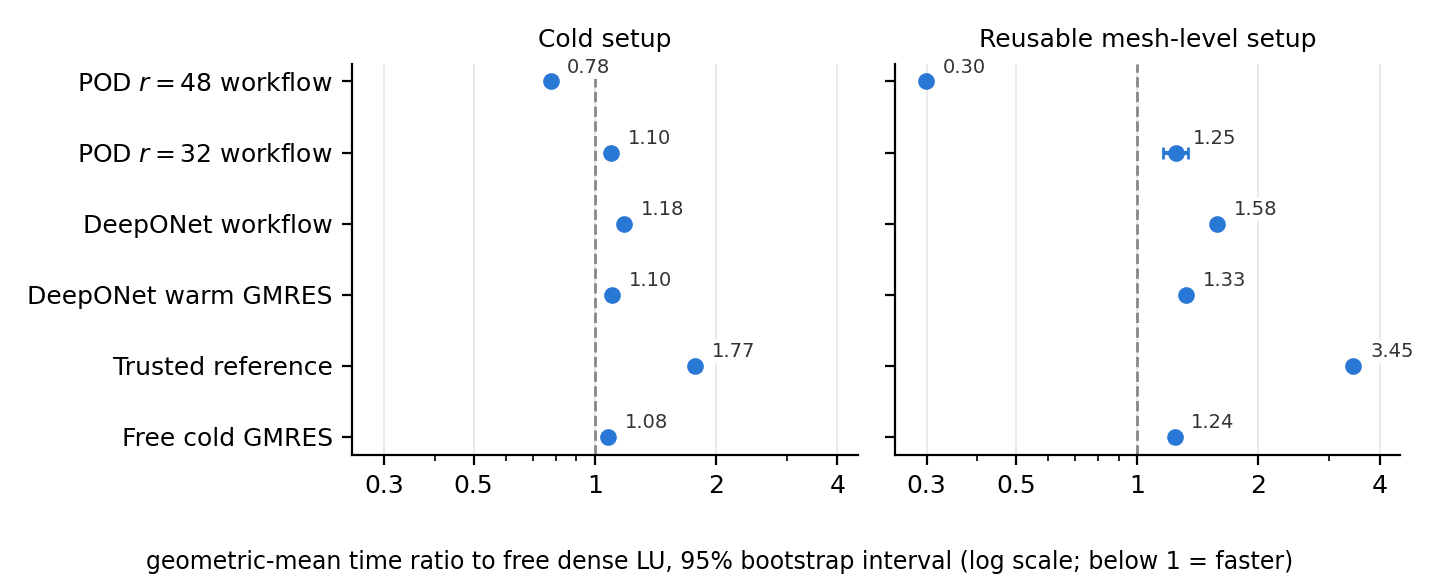
\includegraphics[width=0.94\linewidth]{figures/benchmark_ratios.png}
\caption{Trajectory benchmark: geometric-mean time ratio to free dense LU
with query-bootstrap intervals. All plotted methods meet the target on
120/120 queries; the raw neural candidate meets it on none.}
\label{fig:benchmark-ratios}
\end{figure}
The ratios are geometric means of paired query times on common accepted
queries. The one-time mesh setup is about 0.57 s for all methods; amortising
it over 120 queries preserves these conclusions. Rank-48 POD has an online
advantage beginning with the first query \emph{given an available basis}.
This comparison excludes the cost of generating data and constructing the
basis.

The terminal-price benchmark has the same acceptance counts. Independent
COS prices approximate the continuum target; they lie within \$0.01 of the
stored coarse-grid price on 9 of 120 queries, with median difference
\$0.031 and maximum \$0.31. This measures the distinct price targets, so
COS timings are not compared under the discrete target.

\subsection{POD rank and acceptance}
\label{ssec:pod-results}
\begin{table}[!htbp]
\centering\small
\caption{Mass-weighted POD baseline on the fixed 30-query validation set (training: 800 assembled trajectories, 48{,}800 uncentred free snapshots). Errors in the $M_I$ norm against the stored reference: projection and $E_{\rm rel}$ are maxima over time, $\beta_0$ is the finite-rank initial error. Single-valued error and bound columns are query medians; $E_{\rm rel}$ gives median and maximum. Last column: direct / corrected acceptance at $10^{-3}$ through the assembled free workflow (all 30 delivered).}
\label{tab:repaired-pod}
\resizebox{\textwidth}{!}{%
\begin{tabular}{lrrrrrrr}
\toprule
basis & $r$ & projection & $\beta_0$ & $E_{\rm rel}$ med./max & price err. (\$) & cand. $\eta_{\rm aug}$ & dir./corr.\\
\midrule
mass-weighted & 8 & $0.332$ & $0.332$ & $1.33\times10^{-3}$ / $4.17\times10^{-3}$ & $0.0395$ & $2.96$ & 0/30\\
mass-weighted & 16 & $0.0235$ & $0.0235$ & $1.05\times10^{-4}$ / $4.37\times10^{-4}$ & $4.57\times10^{-4}$ & $0.252$ & 0/30\\
mass-weighted & 32 & $3.34\times10^{-4}$ & $1.44\times10^{-4}$ & $1.36\times10^{-6}$ / $3.40\times10^{-6}$ & $1.14\times10^{-6}$ & $1.58\times10^{-3}$ & 0/30\\
mass-weighted & 48 & $4.16\times10^{-6}$ & $7.65\times10^{-7}$ & $1.72\times10^{-8}$ / $5.57\times10^{-8}$ & $1.66\times10^{-8}$ & $1.63\times10^{-5}$ & 30/0\\
mass-weighted & 62 & $2.58\times10^{-13}$ & $2.02\times10^{-13}$ & $1.06\times10^{-9}$ / $6.13\times10^{-9}$ & $1.54\times10^{-8}$ & $3.40\times10^{-11}$ & 30/0\\
\bottomrule
\end{tabular}}
\par\smallskip\parbox{0.95\linewidth}{\footnotesize Full-rank recovery against a dense direct solve of the same free CN system: 46/46 within the residual-derived allowance (30 validation queries, 8 exact vertices, 8 selected full-space failures; max error/allowance 0.011, max relative coefficient error $5.1\times10^{-14}$).}
\end{table}

On the separate 30-query validation set, mass-weighted POD at ranks 48 and
62 passes directly on every query, whereas ranks 8, 16 and 32 require
correction (Table~\ref{tab:repaired-pod}). At rank 32 the median initial
error is $1.44\times10^{-4}$, below the tolerance, but the median augmented
bound is $1.58\times10^{-3}$. The rejection therefore cannot be attributed
to the initial term alone. Full-rank recovery agrees with a dense solve of
the free CN system within its residual-derived allowance on all 46 tested
queries, including validation points, vertices and selected full-space
failure cases. A mass-orthonormalised Euclidean-SVD comparison has similar
errors; neither basis dominates the validation maxima. Its rank-32 model
passes directly on four queries. Mass weighting is optimal for the training
snapshot objective, rather than for every validation trajectory.

\subsection{Solver and certification costs under refinement}
\label{ssec:scaling-results}
\begin{table}[!htbp]
\centering\small
\caption{Cold solver and certificate costs under refinement (60 CN steps,
single thread; 30 queries at $N\le256$, six at $N=512$; three repetitions).
Times are query medians of repetition medians. The lower-bound column is
spectral setup; Riesz includes residual evaluation and PCG. Counts include
all timed repetitions; memory is peak traced allocation.}
\label{tab:scaling}
\textit{Timing phases (seconds).}\par\smallskip
\begin{tabular}{rlrrrrr}
\toprule
$N$ & Method & Total & Assembly & Advance & Lower bound & Riesz\\
\midrule
64 & Iterative reference & $1.47$ & $0.56$ & $0.649$ & $0.005$ & $0.25$\\
64 & Dense LU & $0.83$ & $0.56$ & $0.004$ & $0.005$ & $0.25$\\
64 & GMRES & $0.89$ & $0.56$ & $0.069$ & $0.005$ & $0.25$\\
128 & Iterative reference & $2.86$ & $1.14$ & $1.237$ & $0.013$ & $0.47$\\
128 & Dense LU & $1.65$ & $1.14$ & $0.007$ & $0.013$ & $0.47$\\
128 & GMRES & $1.70$ & $1.14$ & $0.063$ & $0.013$ & $0.47$\\
256 & Iterative reference & $5.75$ & $2.27$ & $2.399$ & $0.040$ & $1.02$\\
256 & Dense LU & $3.37$ & $2.28$ & $0.015$ & $0.040$ & $1.01$\\
256 & GMRES & $3.43$ & $2.28$ & $0.068$ & $0.040$ & $1.01$\\
512 & Iterative reference & $14.76$ & $4.59$ & $4.856$ & $0.284$ & $5.00$\\
512 & Dense LU & $10.02$ & $4.58$ & $0.102$ & $0.282$ & $5.01$\\
512 & GMRES & $10.08$ & $4.58$ & $0.183$ & $0.281$ & $5.01$\\
\bottomrule
\end{tabular}
\par\smallskip\textit{Dimensions, acceptance and iteration counts.}\par\smallskip
\begin{tabular}{rrlrrr}
\toprule
$N$ & Stored dof & Method & Verified runs & PCG it. & MB\\
\midrule
64 & 66 & Iterative reference & 90/90 & 2948 & $0.4$\\
64 & 66 & Dense LU & 90/90 & 2942 & $0.3$\\
64 & 66 & GMRES & 90/90 & 2942 & $0.3$\\
128 & 130 & Iterative reference & 90/90 & 4870 & $1.0$\\
128 & 130 & Dense LU & 90/90 & 4864 & $1.0$\\
128 & 130 & GMRES & 90/90 & 4868 & $1.0$\\
256 & 258 & Iterative reference & 90/90 & 8189 & $3.3$\\
256 & 258 & Dense LU & 90/90 & 8160 & $3.1$\\
256 & 258 & GMRES & 90/90 & 8172 & $3.1$\\
512 & 514 & Iterative reference & 18/18 & 12000 & $11.5$\\
512 & 514 & Dense LU & 18/18 & 12000 & $11.3$\\
512 & 514 & GMRES & 18/18 & 12000 & $11.3$\\
\bottomrule
\end{tabular}
\end{table}

The cost study refines the deterministic solve and certificate, with 60 CN
steps held fixed. The neural and POD approximations are evaluated only at
$N=64$. Table~\ref{tab:scaling} and Figure~\ref{fig:scaling} show approximately
linear growth in total cost up to $N=256$. Assembly and certification
 dominate the optimised free solvers; advancement contributes below 8\%
of their total cost, versus 33--44\% for the iterative reference.
At $N=512$, certification grows to about 5 s and every time step reaches
the 200-iteration PCG cap. The bracket remains an upper bound under its
spectral hypothesis, and the computed certificate passes on all 18 timed
runs. Efficient fine-mesh certification therefore requires cheaper spectral
bounds and Riesz evaluation.

\begin{figure}[!htbp]
\centering
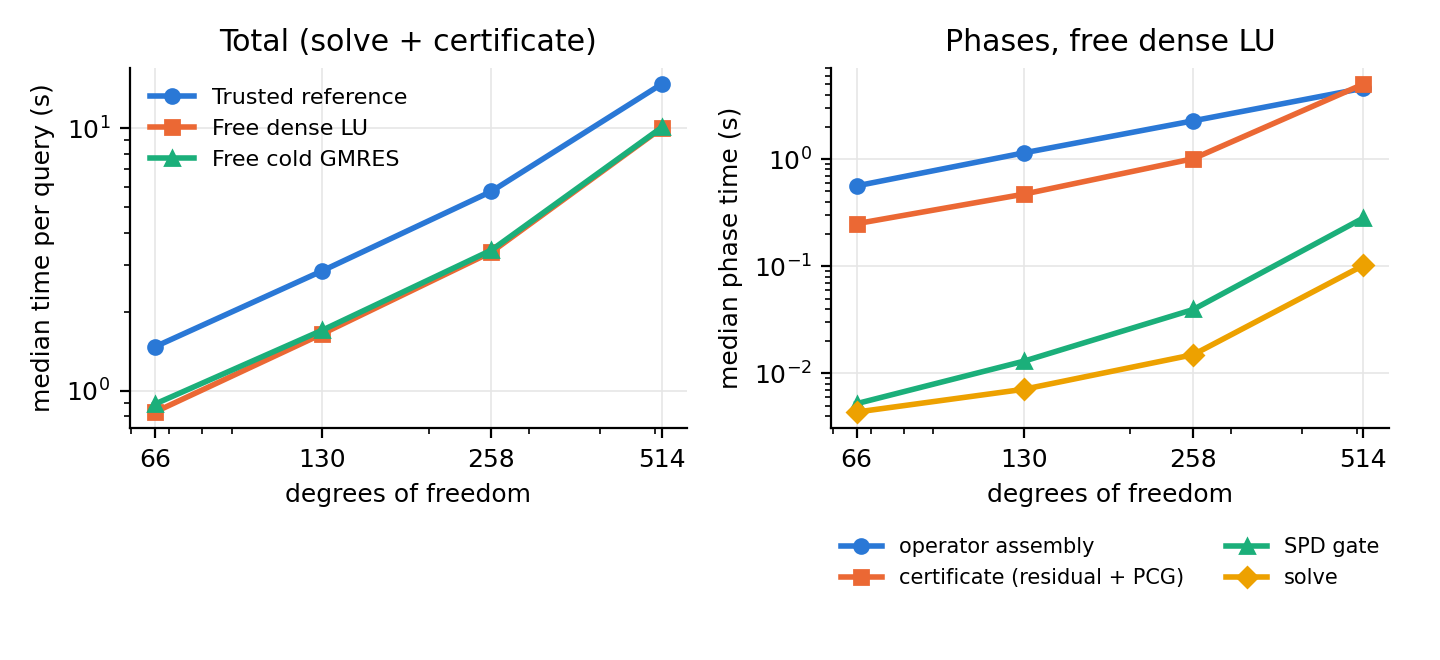
\includegraphics[width=0.94\linewidth]{figures/scaling.png}
\caption{Cold solver and certificate cost under spatial refinement. Left:
median total time. Right: phase medians for free dense LU. The study uses
30 queries for $N\le256$ and six for $N=512$, with three repetitions.}
\label{fig:scaling}
\end{figure}

\subsection{Assembly and continuum-price diagnostics}
\label{ssec:refinement}\label{ssec:fourier-financial}
Table~\ref{tab:assembly} distinguishes agreement with the principal-period
rule from agreement with the exact real-line Galerkin integral.
Independent 40-digit quadrature of the principal-period integral gives
entrywise differences decreasing from about $10^{-3}$ at $N=64$ to
$10^{-5}$ at $N=512$, with virtually unchanged free positivity decisions.
Against real-line Galerkin coefficients, the relative operator-norm
difference is 33--41\%, concentrated at high frequencies and persisting
under refinement. The minimum free eigenvalue changes by less than
$9\times10^{-4}$ relatively in those tests. Thus numerical algebraic
positivity and exact variational assembly remain distinct properties.

\begin{table}[!htbp]
\centering\small
\caption{Independent 40-digit assembly comparisons: quadrature of the
principal-period convention and exact real-line Galerkin coefficients.
Relative errors; ten cost-study queries for $N\le256$, three for $N=512$.
The eigenvalue column is maximum relative change in $\lambda_{\min}(S_I)$.}
\label{tab:assembly}
\textit{Evolution-matrix differences.}\par\smallskip
\begin{tabular}{lrrrr}
\toprule
Comparator & $N$ & Queries & Max entry $A$ & Operator norm med./max\\
\midrule
Principal period & 64 & 10 & $1.03\times10^{-3}$ & $6.95\times10^{-3}$ / $0.0135$\\
Principal period & 128 & 10 & $2.59\times10^{-4}$ & $3.26\times10^{-3}$ / $6.23\times10^{-3}$\\
Principal period & 256 & 10 & $6.34\times10^{-5}$ & $1.55\times10^{-3}$ / $2.92\times10^{-3}$\\
Principal period & 512 & 3 & $1.22\times10^{-5}$ & $1.00\times10^{-3}$ / $1.11\times10^{-3}$\\
Real line & 64 & 10 & $0.108$ & $0.382$ / $0.412$\\
Real line & 128 & 10 & $0.105$ & $0.371$ / $0.408$\\
Real line & 256 & 10 & $0.102$ & $0.358$ / $0.405$\\
Real line & 512 & 3 & $0.101$ & $0.333$ / $0.402$\\
\bottomrule
\end{tabular}
\par\smallskip\textit{Mass matrix and positivity.}\par\smallskip
\begin{tabular}{lrrrrr}
\toprule
Comparator & $N$ & Queries & Max entry $M$ & Eigenvalue change & Positivity agrees\\
\midrule
Principal period & 64 & 10 & $4.0\times10^{-16}$ & $4.1\times10^{-7}$ & 10/10\\
Principal period & 128 & 10 & $4.0\times10^{-16}$ & $6.0\times10^{-8}$ & 10/10\\
Principal period & 256 & 10 & $3.0\times10^{-15}$ & $8.3\times10^{-9}$ & 10/10\\
Principal period & 512 & 3 & $7.9\times10^{-15}$ & $9.4\times10^{-10}$ & 3/3\\
Real line & 64 & 10 & $4.0\times10^{-16}$ & $8.9\times10^{-4}$ & 10/10\\
Real line & 128 & 10 & $4.0\times10^{-16}$ & $4.4\times10^{-4}$ & 10/10\\
Real line & 256 & 10 & $3.0\times10^{-15}$ & $2.2\times10^{-4}$ & 10/10\\
Real line & 512 & 3 & $7.9\times10^{-15}$ & $1.1\times10^{-4}$ & 3/3\\
\bottomrule
\end{tabular}
\end{table}


Independent COS and Carr--Madan prices agree to $4\times10^{-13}$ on all
150 price-diagnostic rows at the extended settings: COS uses 8192 modes
and range parameter 30, and Carr--Madan has cutoff cap 51,200. A 60-digit
Carr--Madan calculation reproduces the worst-case 40-digit checks.
This is convergence evidence for the reference prices, rather than an
error enclosure.

\begin{table}[!htbp]
\centering\small
\caption{Refinement of the assembled discrete price (first 8 price-diagnostic queries; spots $0.8K..1.2K$, maximum within query, then median over queries). Paired difference $=\max_s|V_k-V_{k+1}|$ to the next level; COS gap is an independent continuum diagnostic. Space: $h=16/N$, 480 steps; time: $N=1024$; domain: $h=0.125$ fixed, half-width $L$.}
\label{tab:refinement}
\begin{tabular}{lrrrrr}
\toprule
study & $N$ & steps & $L$ & paired diff. (\$) & COS gap (\$)\\
\midrule
space & 64 & 480 & $8$ & $0.0233$ & $0.0215$\\
space & 128 & 480 & $8$ & $5.39\times10^{-3}$ & $5.37\times10^{-3}$\\
space & 256 & 480 & $8$ & $1.08\times10^{-3}$ & $1.15\times10^{-3}$\\
space & 512 & 480 & $8$ & $2.40\times10^{-4}$ & $1.94\times10^{-4}$\\
space & 1024 & 480 & $8$ & -- & $5.05\times10^{-5}$\\
time & 1024 & 15 & $8$ & $0.0411$ & $0.0413$\\
time & 1024 & 30 & $8$ & $5.71\times10^{-4}$ & $7.65\times10^{-4}$\\
time & 1024 & 60 & $8$ & $1.43\times10^{-4}$ & $2.01\times10^{-4}$\\
time & 1024 & 120 & $8$ & $3.59\times10^{-5}$ & $7.35\times10^{-5}$\\
time & 1024 & 240 & $8$ & $8.96\times10^{-6}$ & $4.84\times10^{-5}$\\
time & 1024 & 480 & $8$ & $2.13\times10^{-6}$ & $5.05\times10^{-5}$\\
time & 1024 & 960 & $8$ & -- & $5.04\times10^{-5}$\\
domain & 96 & 240 & $6$ & $1.87\times10^{-3}$ & $6.71\times10^{-3}$\\
domain & 128 & 240 & $8$ & $9.05\times10^{-4}$ & $5.37\times10^{-3}$\\
domain & 160 & 240 & $10$ & $6.01\times10^{-4}$ & $4.67\times10^{-3}$\\
domain & 192 & 240 & $12$ & -- & $4.15\times10^{-3}$\\
\bottomrule
\end{tabular}
\end{table}

Spatial differences approach second-order decay, and temporal differences
at $N=1024$ decrease at second order once the coarse startup regime is
passed (Table~\ref{tab:refinement}). The refined gap to COS levels off near
$5\times10^{-5}$. At fixed $h=0.125$, changing domain half-width from 6 to
12 still changes the COS gap by about $2.5\times10^{-3}$, leaving domain
sensitivity unresolved at that resolution.

\begin{table}[!htbp]
\centering\small
\caption{Corner discrepancy diagnostic (240 time steps; the $N=64$ values are unchanged with 60 steps). Corner A/0397: $C=0.05$, $Y=1.1$, $T=0.1$, $r=0.01$. Spots $0.8K..1.2K$.}
\label{tab:corner}
\begin{tabular}{lrrrr}
\toprule
query & $N$ & $\max_s|V_h(T)-\mathrm{COS}|$ & $\max_s|V_h(0)-\psi|$ & $\min_s V_h(T)$\\
\midrule
Corner A & 64 & $2.22$ & $3.30$ & $-1.17$\\
Corner A & 128 & $0.774$ & $1.66$ & $-0.357$\\
Corner A & 256 & $0.195$ & $0.829$ & $0.0225$\\
Corner A & 512 & $0.0275$ & $0.415$ & $0.0489$\\
Corner A & 1024 & $1.61\times10^{-3}$ & $0.207$ & $0.0474$\\
Corner B & 64 & $2.07$ & $3.30$ & $-1.11$\\
Corner B & 128 & $0.693$ & $1.66$ & $-0.293$\\
Corner B & 256 & $0.164$ & $0.829$ & $0.0379$\\
Corner B & 512 & $0.0200$ & $0.415$ & $0.0517$\\
Corner B & 1024 & $8.34\times10^{-4}$ & $0.207$ & $0.0510$\\
Interior query & 64 & $0.107$ & $3.30$ & $3.48$\\
Interior query & 128 & $8.46\times10^{-3}$ & $1.66$ & $3.58$\\
Interior query & 256 & $6.71\times10^{-4}$ & $0.829$ & $3.58$\\
Interior query & 512 & $1.65\times10^{-4}$ & $0.415$ & $3.58$\\
Interior query & 1024 & $2.82\times10^{-5}$ & $0.207$ & $3.58$\\
\bottomrule
\end{tabular}
\end{table}

Two short-maturity, weakly diffusive box corners have coarse-grid price
gaps exceeding \$2, with negative values at some spots. Spatial refinement
reduces these gaps to roughly $10^{-3}$ at $N=1024$, whereas time refinement
alone leaves them unchanged. The initial payoff projection error also
 decreases with mesh size. These observations are consistent with inadequate
spatial resolution, but do not isolate the propagated contribution of
initial projection alone. The algebraic certificate can remain valid while
the underlying discrete price is a poor continuum approximation.

\begin{table}[!htbp]
\centering\small
\caption{Financial budgets on all 30 price-diagnostic queries at five spots (maximum within query; medians over queries). Bounds are $\beta_I(x)\eta_{\rm aug}$ relative to the exact assembled discrete price (exact-arithmetic theorem, floating-point evaluation); the stored-reference and COS columns are diagnostics, the latter including discretisation error.}
\label{tab:financial}
\par\smallskip
\textit{Acceptance and algebraic bounds.}
\par\smallskip
\begin{tabular}{lrrrrr}
\toprule
Model & Delivered & \shortstack{Raw verified\\1/5/10 cents} & \shortstack{Final verified\\1/5/10 cents} & \shortstack{Raw bound\\(\$)} & \shortstack{Final bound\\median / max (\$)}\\
\midrule
DeepONet & 30/30 & 0 / 0 / 0 & 30 / 30 / 30 & $7.36$ & $2.23\times10^{-6}$ / $7.99\times10^{-6}$\\
POD $r=48$ & 30/30 & 30 / 30 / 30 & 30 / 30 / 30 & $3.34\times10^{-5}$ & $3.34\times10^{-5}$ / $7.03\times10^{-5}$\\
\bottomrule
\end{tabular}
\par\smallskip
\textit{Reference and continuum diagnostics.}
\par\smallskip
\begin{tabular}{lrrr}
\toprule
Model & \shortstack{Reference allowance\\(\$)} & \shortstack{Difference to stored reference\\(\$)} & \shortstack{Difference to COS\\median / max (\$)}\\
\midrule
DeepONet & $2.17\times10^{-6}$ & $6.33\times10^{-8}$ & $0.0297$ / $0.391$\\
POD $r=48$ & $2.17\times10^{-6}$ & $6.31\times10^{-8}$ & $0.0297$ / $0.391$\\
\bottomrule
\end{tabular}
\par\smallskip\parbox{0.95\linewidth}{\footnotesize Window factors on $[\log0.8K,\log1.2K]$ (two mesh cells): sampled maximum of $\beta_I$ 2.199824 (diagnostic); cellwise piecewise-polynomial maximum 2.19982442 (floating-point evaluation, not a validated supremum); window-Gram $L^2$ factor 0.959 (integrated error, kept separate).}
\end{table}

The financial-budget study converts the trajectory bound using
$\beta_I(x)$ (Table~\ref{tab:financial}). Raw neural predictions pass none
of the one-, five- or ten-cent budgets. After correction all 30 queries
pass the one-cent target, with median price bound about
$2.2\times10^{-6}$ dollars. Rank-48 POD passes directly on every query.
The median discrete-to-COS gap is about \$0.03, much larger than these
surrogate bounds.
\FloatBarrier
\section{Interpretation and conclusion}
\label{sec:conclusion}\label{sec:discussion}
The residual framework turns a candidate spline trajectory into a
query-wise bound through the governing discrete equation. Restricting to
the free coefficient space and retaining the initial discrepancy are
necessary for a consistent treatment of neural and reduced trajectories.
The Riesz bracket separates validity from iterative convergence under its
spectral lower-bound hypothesis. The deterministic discretisation supplies
the training data, operator, exterior constraints and correction mechanism;
certification therefore remains anchored in numerical stability.

The benchmark identifies the practical distinction between prediction
accuracy and tolerance-controlled cost. The neural model requires
correction throughout the tested population, while rank-48 POD passes
directly and reduces online time. Assembly and certification dominate the
optimised free solver costs, making their reduction a prerequisite for
larger surrogate gains. This finding applies to the tested resolution,
parameter family and available checkpoints; it establishes neither a
general neural speed advantage nor a lifecycle cost advantage.

Discrete certification and continuum pricing accuracy require separate
assessment. The principal-period matrix differs from exact Galerkin
assembly, and the coarse mesh gives substantial price errors at difficult
corners. Refinement provides empirical convergence evidence, but no
computable continuum-price bound for this assembled scheme. Similarly,
ordinary floating-point checks do not supply machine-enclosed guarantees;
validated spectral bounds and arithmetic would strengthen the implemented
certificate.

The resulting method provides scheme-consistent residual certification of
neural and reduced European-put trajectories, together with a matched
assessment of its online value. Its next computational priorities are
inexpensive fine-mesh spectral bounds, efficient Riesz evaluation and
spatial resolution adequate for the required price budget. Broader payoff
families and mesh-transfer strategies require further evaluation.
\FloatBarrier
\appendix
\section{Uniform stability and supporting derivations}
\label{app:proofs}
\subsection{Explicit constants and proof of uniform stability}
\label{app:proof-uniform}
For the box \eqref{eq:parameter-set}, define
\begin{equation}
  a_\ast:=\max\{M_{\max},G_{\max}\},
  \qquad
  \delta_\ast:=\tfrac{\pi}{4}\bigl(Y_{\min}-1\bigr)>0,
  \qquad
  R_\ast:=a_\ast\tan\!\Bigl(\frac{\pi/2+\delta_\ast}{Y_{\min}}\Bigr).
  \label{eq:uniform-constants-aux}
\end{equation}
Explicit admissible choices are
\begin{equation}
  c_1
  =\frac{1}{1+2\Theta}
  \min\left\{
    \frac{r_{\min}}{(1+R_\ast^2)^{Y_{\max}/2}},\;
    2C_{\min}\gamma_{\min}\sin(\delta_\ast)
    \Bigl(\frac{R_\ast^2}{1+R_\ast^2}\Bigr)^{Y_{\max}/2}
  \right\},
  \label{eq:c1-explicit}
\end{equation}
and
\begin{equation}
  C_{\rm cont}
  =2\Bigl(
    \Omega_\ast
    +2C_{\max}\gamma_{\max}\max\{1,a_\ast^2\}^{Y_{\max}/2}
    +\lambda_\ast
  \Bigr),
  \label{eq:Ccont-explicit}
\end{equation}
where
\begin{equation}
\begin{gathered}
\gamma_{\min}:=\!\!\min_{Y\in[Y_{\min},Y_{\max}]}\!\!\Gamma(-Y)>0,
\qquad
\gamma_{\max}:=\!\!\max_{Y\in[Y_{\min},Y_{\max}]}\!\!\Gamma(-Y)<\infty,
\\
\Theta:=\max\{1,M_{\max}^2,G_{\max}^2\}^{Y_{\max}/2},
\qquad
\Omega_\ast:=\sup_{\mu\in\Pset}|\rf-\omega_S(\mu)|,
\qquad
\lambda_\ast:=\sup_{\mu\in\Pset}\lambda_0(\mu),
\end{gathered}
\label{eq:uniform-aux-constants}
\end{equation}
the last two being finite.
Throughout, $\mu=(C,G,M,Y,\rf)\in\Pset$ and $s_\mu=Y/2\in(1/2,1)$.  We work on
the full line and transfer to $\Omega$ at the end using
Lemma~\ref{lem:conformity} and the zero-extension convention
\eqref{eq:energy-space}, which preserve all constants.

\medskip\noindent
\textbf{Step 1: uniform equivalence of the parameter-dependent norm.}
Let $s\in[Y_{\min}/2,Y_{\max}/2]\subset(1/2,1)$ and let
$w_\mu(\xi):=1+|M-i\xi|^{2s}+|G+i\xi|^{2s}
=1+(M^2+\xi^2)^{s}+(G^2+\xi^2)^{s}$ be the weight in
\eqref{eq:HMG-norm}.  Since $s\le1$ and $(a+b)^s\le a^s+b^s$ for $s\in(0,1]$,
\[
  w_\mu(\xi)\ \le\ 1+2\max\{1,M_{\max}^2,G_{\max}^2\}^{s}(1+\xi^2)^{s}
  \ \le\ (1+2\Theta)(1+\xi^2)^{s},
\]
with $\Theta=\max\{1,M_{\max}^2,G_{\max}^2\}^{Y_{\max}/2}$, using
$(1+\xi^2)^s\ge1$.  For the lower bound, $w_\mu(\xi)\ge1+|\xi|^{2s}$ and,
since $(1+\xi^2)^s\le2^s\max\{1,|\xi|^{2s}\}\le2(1+|\xi|^{2s})$ for
$s\le1$,
\[
  w_\mu(\xi)\ \ge\ \tfrac12(1+\xi^2)^{s}.
\]
Hence, uniformly in $\mu\in\Pset$,
\begin{equation}
  \tfrac12\norm{u}_{H^{s_\mu}(\R)}^2
  \ \le\ \norm{u}_{H^{s_\mu}_{M,G}(\R)}^2
  \ \le\ (1+2\Theta)\norm{u}_{H^{s_\mu}(\R)}^2 ,
  \label{eq:uniform-norm-equivalence}
\end{equation}
where $\norm{u}_{H^{s}(\R)}^2=\tfrac1{2\pi}\int(1+\xi^2)^{s}|\widehat u|^2$.

\medskip\noindent
\textbf{Step 2: uniform continuity.}
From \eqref{eq:symbol}, for every $\xi$,
\[
  |A_\mu(\xi)|
  \le|\rf-\omega_S||\xi|
   +C\Gamma(-Y)\bigl[(M^2+\xi^2)^{Y/2}+(G^2+\xi^2)^{Y/2}\bigr]
   +\lambda_0 .
\]
The map $(C,G,M,Y)\mapsto\omega_S$ of \eqref{eq:martingale-correction} is
continuous on $\Pset$ because $(M-1)^Y$ is continuous and finite on the selected box
(and remains so at $M=1$), and $\Gamma(-Y)$ is continuous on $[Y_{\min},Y_{\max}]\subset(1,2)$;
hence $\Omega_\ast<\infty$ and $\lambda_\ast<\infty$.  Since $Y>1$ we have
$|\xi|\le(1+\xi^2)^{Y/2}$, and
$(a^2+\xi^2)^{Y/2}\le\max\{1,a^2\}^{Y/2}(1+\xi^2)^{Y/2}$.  Therefore
\begin{equation}
  |A_\mu(\xi)|
  \le\Bigl(\Omega_\ast+2C_{\max}\gamma_{\max}\max\{1,a_\ast^2\}^{Y_{\max}/2}
   +\lambda_\ast\Bigr)(1+\xi^2)^{s_\mu}.
  \label{eq:uniform-symbol-upper}
\end{equation}
By Plancherel's theorem and the Cauchy--Schwarz inequality,
\[
  |a_\R(u,w)|
  \le\Bigl(\sup_{\xi\in\R}\frac{|A_\mu(\xi)|}{(1+\xi^2)^{s_\mu}}\Bigr)
  \norm{u}_{H^{s_\mu}(\R)}\norm{w}_{H^{s_\mu}(\R)},
\]
and
\eqref{eq:uniform-norm-equivalence} converts the $H^{s_\mu}$ norms into
$H^{s_\mu}_{M,G}$ norms at the cost of a factor $2$.  This gives
\eqref{eq:Ccont-explicit}.

\medskip\noindent
\textbf{Step 3: the zero-frequency and low-frequency region.}
By the exact identity \eqref{eq:symbol-real-exact}, $\Gamma(-Y)>0$ for
$Y\in(1,2)$, and the monotonicity $\Real(a\pm i\xi)^Y\le a^Y$ of
\cite{DamircheliCGMY2026}, both bracketed terms in
\eqref{eq:symbol-real-exact} are nonnegative, so
\begin{equation}
  \Real A_\mu(\xi)\ \ge\ \rf\ \ge\ r_{\min}>0
  \qquad\text{for all }\xi\in\R,\ \mu\in\Pset .
  \label{eq:uniform-low-freq}
\end{equation}
This is where $r_{\min}>0$ is used, and it is the only place: at $\xi=0$ the
fractional contribution vanishes identically.

\medskip\noindent
\textbf{Step 4: a uniform high-frequency lower bound.}
Write $\Real(a\pm i\xi)^Y=(a^2+\xi^2)^{Y/2}\cos\bigl(Y\vartheta_a(\xi)\bigr)$
with $\vartheta_a(\xi)=\arctan(|\xi|/a)\in[0,\pi/2)$.  Recall
$\delta_\ast=\tfrac\pi4(Y_{\min}-1)>0$ and
$\vartheta_\ast:=(\pi/2+\delta_\ast)/Y_{\min}$.  Since
$Y_{\min}>1$ we have
\[
  \vartheta_\ast
  =\frac{\pi/2+\tfrac\pi4(Y_{\min}-1)}{Y_{\min}}
  =\frac{\pi}{4}\cdot\frac{Y_{\min}+1}{Y_{\min}}
  <\frac{\pi}{2},
\]
because $Y_{\min}+1<2Y_{\min}$.  Hence $R_\ast=a_\ast\tan\vartheta_\ast$ is
finite and positive.  Let $|\xi|\ge R_\ast$ and let $a\in\{M,G\}$, so that
$a\le a_\ast$ and therefore
$\vartheta_a(\xi)=\arctan(|\xi|/a)\ge\arctan(R_\ast/a_\ast)=\vartheta_\ast$.
Consequently
\[
  Y\vartheta_a(\xi)\ \ge\ Y_{\min}\vartheta_\ast=\frac\pi2+\delta_\ast,
  \qquad
  Y\vartheta_a(\xi)\ <\ Y\cdot\frac\pi2\ <\ \pi ,
\]
the last inequality because $Y<2$.  As $\cos$ is decreasing on
$[\pi/2,\pi]$,
\[
  \cos\bigl(Y\vartheta_a(\xi)\bigr)\ \le\ \cos\Bigl(\frac\pi2+\delta_\ast\Bigr)
  =-\sin\delta_\ast\ <\ 0 .
\]
Therefore, for $|\xi|\ge R_\ast$,
$\Real\bigl[(M-i\xi)^Y+(G+i\xi)^Y\bigr]\le-2\sin(\delta_\ast)|\xi|^Y$, using
$(a^2+\xi^2)^{Y/2}\ge|\xi|^Y$.  Since the drift term in \eqref{eq:symbol} is
purely imaginary and $\lambda_0>0$,
\begin{equation}
  \Real A_\mu(\xi)
  \ \ge\ 2C\Gamma(-Y)\sin(\delta_\ast)|\xi|^Y
  \ \ge\ \kappa_\ast|\xi|^{Y},
  \qquad |\xi|\ge R_\ast,
  \label{eq:uniform-high-freq}
\end{equation}
with $\kappa_\ast:=2C_{\min}\gamma_{\min}\sin\delta_\ast>0$, where
$\gamma_{\min}=\min_{[Y_{\min},Y_{\max}]}\Gamma(-Y)>0$ by continuity and
positivity of $\Gamma(-\cdot)$ on $(1,2)$.  Note that $\delta_\ast$, and hence
$\kappa_\ast$, degenerate as $Y_{\min}\downarrow1$; this is the analytic
content of the requirement $Y_{\min}>1$.

\medskip\noindent
\textbf{Step 5: combination.}
For $|\xi|\le R_\ast$, \eqref{eq:uniform-low-freq} and
$(1+\xi^2)^{s_\mu}\le(1+R_\ast^2)^{Y_{\max}/2}$ give
$\Real A_\mu(\xi)\ge r_{\min}(1+R_\ast^2)^{-Y_{\max}/2}(1+\xi^2)^{s_\mu}$.
For $|\xi|\ge R_\ast$, since $t\mapsto t^2/(1+t^2)$ is increasing and
$\bigl(R_\ast^2/(1+R_\ast^2)\bigr)^{Y/2}
\ge\bigl(R_\ast^2/(1+R_\ast^2)\bigr)^{Y_{\max}/2}$,
\[
  \frac{|\xi|^{Y}}{(1+\xi^2)^{Y/2}}
  =\Bigl(\frac{\xi^2}{1+\xi^2}\Bigr)^{Y/2}
  \ \ge\ \Bigl(\frac{R_\ast^2}{1+R_\ast^2}\Bigr)^{Y_{\max}/2},
\]
so \eqref{eq:uniform-high-freq} gives
$\Real A_\mu(\xi)\ge\kappa_\ast(R_\ast^2/(1+R_\ast^2))^{Y_{\max}/2}(1+\xi^2)^{s_\mu}$.
Taking the minimum of the two prefactors and applying Plancherel's theorem,
\[
  \Real a_\R(u,u)\ \ge\ \tilde c_1\norm{u}_{H^{s_\mu}(\R)}^2,
  \qquad
  \tilde c_1
  =\min\Bigl\{\tfrac{r_{\min}}{(1+R_\ast^2)^{Y_{\max}/2}},\
   \kappa_\ast\bigl(\tfrac{R_\ast^2}{1+R_\ast^2}\bigr)^{Y_{\max}/2}\Bigr\},
\]
and \eqref{eq:uniform-norm-equivalence} converts this into the
$H^{s_\mu}_{M,G}$ norm at the cost of the factor $(1+2\Theta)^{-1}$, giving
\eqref{eq:c1-explicit}.

\medskip\noindent
\textbf{Step 6: transfer to $\Omega$.}
For $v,w\in\Vmu$ the zero extensions satisfy
$\widetilde v,\widetilde w\in H^{s_\mu}(\R)$ with
$\norm{\widetilde v}_{L^2(\R)}=\norm{v}_{L^2(\Omega)}$, and by definition
$a_\mu(v,w)=a_\R(\widetilde v,\widetilde w)$ and
$\norm{v}_{\Vmu}=\norm{\widetilde v}_{H^{s_\mu}_{M,G}(\R)}$.  Both estimates
therefore transfer with identical constants, independent of $h$ and of
$\Omega$.  Finally, for real-valued $v$ the form $a_\mu(v,v)$ is real, so
$a_\mu(v,v)=\Real a_\mu(v,v)$.  \qed


The constants are explicit admissible choices rather than optimal ones.
On the reported box their approximate values are
$c_1\approx1.576\times10^{-8}$ and
$C_{\rm cont}\approx2.525\times10^3$, illustrating conservatism.
These evaluations are not validated enclosures; the theorem uses the
analytically defined extrema.

\subsection{Exact-assembly consequences and constrained dual norms}
\label{ssec:exact-assembly}\label{lem:Sh-spd}\label{eq:Sh-spd}
Under exact assembly, $z^\top\Sh z=a_\mu(z_h,z_h)$, so uniform coercivity
implies $\Sh\succ0$. The symmetric parts of $\Mh+\dt\Ah/2$ and
$\Mh+\dt\Ah$ are positive definite, giving nonsingularity.
\begin{lemma}[Positive-rate mass lower bound for exact assembly]
\label{lem:mass-lower}
Under the exact-assembly hypothesis of Lemma~\ref{lem:Sh-spd}, for
$\mu\in\Pset$ (so $\rf>0$),
\begin{equation}
  \Sh(\mu)\succeq \rf\,\Mh
  \label{eq:S-ge-rM}
\end{equation}
in the Loewner order, and consequently
\begin{equation}
  \bb^\top\Sh(\mu)^{-1}\bb\le \rf^{-1}\,\bb^\top\Mh^{-1}\bb
  \qquad\text{for every }\bb\in\R^{N_h}.
  \label{eq:mass-upper}
\end{equation}
\end{lemma}

\begin{proof}
By Lemma~\ref{lem:conformity} and Plancherel's theorem,
\[
  \zz^\top\Sh\zz=a_\mu(z_h,z_h)=a_\R(\widetilde z_h,\widetilde z_h)
  =\frac1{2\pi}\int_\R\Real A_\mu(\xi)\,\bigl|\widehat{\widetilde z_h}(\xi)\bigr|^2\,d\xi .
\]
The exact symbol identity of \cite{DamircheliCGMY2026}, namely
\begin{equation}
\Real A_\mu(\xi)
=\rf+C\Gamma(-Y)\Bigl[\bigl(M^Y-\Real(M-i\xi)^Y\bigr)
+\bigl(G^Y-\Real(G+i\xi)^Y\bigr)\Bigr],
\label{eq:symbol-real-exact}
\end{equation}
together with $\Gamma(-Y)>0$ for $Y\in(1,2)$ and the monotonicity
$\Real(a\pm i\xi)^Y\le a^Y$, gives $\Real A_\mu(\xi)\ge \rf$ for all $\xi$.  Hence
\[
  \zz^\top\Sh\zz\ \ge\ \rf\norm{\widetilde z_h}^2_{L^2(\R)}
  =\rf\norm{z_h}^2_{L^2(\Omega)}=\rf\,\zz^\top\Mh\zz .
\]
Inversion of the Loewner
inequality between positive definite matrices reverses it, giving
\eqref{eq:mass-upper}.
\end{proof}
Exact assembly also implies the mesh-uniform bound on $\kappa_h$:
\[
 \|\Ah v\|_{\Sh^{-1}}
 =\sup_{w\ne0}\frac{a_\mu(v_h,w_h)}{\|w\|_{\Sh}}
 \le\frac{C_{\rm cont}}{c_1}\|v\|_{\Sh}.
\]
For any assembled matrix with SPD symmetric part, duality gives
$\|\Ah v\|_{\Sh^{-1}}\ge v^\top\Ah v/\|v\|_{\Sh}=\|v\|_{\Sh}$,
proving $\kappa_h\ge1$. This quantity is an operator norm, rather than the
condition number of $\Sh$.
\begin{proposition}[Conservatism of a full-space dual norm]
\label{prop:full-space-conservative}
Suppose $\bar S\succ0$, and the reference and candidate have identical
prescribed coefficients. Then $S_I\succ0$ and
\begin{equation}
 \rho_I^\top S_I^{-1}\rho_I
 \le (E\rho_I)^\top\bar S^{-1}(E\rho_I).
 \label{eq:full-space-conservative}
\end{equation}
Consequently a valid upper Riesz bracket for the zero-padded free residual
using $\bar S$ is also a conservative reliability bound for the constrained
problem, subject to the same initial-error and arithmetic assumptions.
\end{proposition}
\begin{proof}
The dual quadratic form equals
$\sup_v(2r^\top v-v^\top S v)$. Restricting the full-space supremum to
$v=Ew$ yields the free-space supremum, proving
\eqref{eq:full-space-conservative}. Positive definiteness restricts to every
principal subspace.
\end{proof}
The converse positivity implication fails because prescribed directions
can make $\bar S$ indefinite while $S_I$ is positive. The entire residual,
Riesz action and spectral bound must use the same constrained space.

\subsection{Discrete parameter stability}
\label{ssec:solution-operator}
\begin{proposition}[Discrete parameter stability of the solution map]
\label{prop:discrete-lipschitz}
Fix a mesh, a time grid, and a payoff $\psi$. Assume that the first
assembled symmetric matrix $\Sh(\mu_1)$ is positive definite, and let
$\mu_1,\mu_2\in\Pset$
with $\cc_h(\mu_1),\cc_h(\mu_2)$ the corresponding Crank--Nicolson
trajectories of \eqref{eq:cn-reference}.  Then, for every
$m=1,\dots,N_T$,
\begin{equation}
\begin{aligned}
  \norm{\cc_h^m(\mu_1)-\cc_h^m(\mu_2)}_{\Mh}^2
  \le{}& \norm{\cc_h^0(\mu_1)-\cc_h^0(\mu_2)}_{\Mh}^2\\
  &+\dt\sum_{n=0}^{m-1}
  \bigl\lVert\bm\varrho^{\,n+1/2}\bigr\rVert_{\Sh(\mu_1)^{-1}}^2 ,
\end{aligned}
  \label{eq:discrete-lipschitz}
\end{equation}
where the parameter-perturbation residual is
\begin{equation}
  \bm\varrho^{\,n+1/2}
  :=\bigl(\Ah(\mu_1)-\Ah(\mu_2)\bigr)\overline\cc_h^{\,n+1/2}(\mu_2)
   -\bigl(\overline\ff^{\,n+1/2}(\mu_1)-\overline\ff^{\,n+1/2}(\mu_2)\bigr).
  \label{eq:param-residual}
\end{equation}
Under exact assembly of the conforming variational matrices,
Theorem~\ref{thm:uniform-coercivity} additionally gives
\begin{equation}
  \norm{\bigl(\Ah(\mu_1)-\Ah(\mu_2)\bigr)\vv}_{\Sh(\mu_1)^{-1}}
  \le
  \frac{1}{c_1}\,
  \sup_{0\ne v_h,w_h\in\Vh}
  \frac{|a_{\mu_1}(v_h,w_h)-a_{\mu_2}(v_h,w_h)|}
       {\norm{v_h}_{\Vp{\mu_1}}\norm{w_h}_{\Vp{\mu_1}}}\;
  \norm{\vv}_{\Sh(\mu_1)},
  \label{eq:matrix-difference}
\end{equation}
so a bound on the difference of the two bilinear forms in a \emph{single}
norm---that of $\mu_1$---suffices, and no common energy space is needed.
\end{proposition}

\begin{proof}
The difference $\ee^n:=\cc_h^n(\mu_1)-\cc_h^n(\mu_2)$ satisfies the
Crank--Nicolson error equation \eqref{eq:discrete-error-equation} with
$\rr_\theta^{n+1/2}$ replaced by $\bm\varrho^{\,n+1/2}$ of
\eqref{eq:param-residual}, since $\cc_h(\mu_2)$ solves the $\mu_2$ scheme
exactly.  Apply Theorem~\ref{thm:fully-discrete-certificate} with
$\Sh=\Sh(\mu_1)$.  Estimate \eqref{eq:matrix-difference} follows from
the continuity argument above applied to the bilinear form
$a_{\mu_1}-a_{\mu_2}$.
\end{proof}
This fixed-grid statement compares both trajectories in the norm of the
first parameter. A continuum regularity result across varying $Y$ would
require additional control of the changing energy spaces.

\subsection{Other time schemes and exponential shifts}
\label{ssec:semidiscrete}\label{ssec:be-certificate}\label{ssec:shifted}
The following extensions follow the same energy argument as
Theorem~\ref{thm:fully-discrete-certificate}.
For a differentiable candidate and a semidiscrete reference, define
$\rho=\Mh\dot\cc_\theta+\Ah\cc_\theta-\ff$. Then
\begin{equation}
 \|\ee(t)\|_{\Mh}^2+\int_0^t\|\ee\|_{\Sh}^2
 \le\|\ee(0)\|_{\Mh}^2+\int_0^t\|\rho\|_{\Sh^{-1}}^2.
 \label{eq:semidiscrete-certificate}
\end{equation}
Multiply the error equation by $\ee^\top$, apply Young's inequality, and
integrate.
For backward Euler, the residual is
$\rho^{n+1}=\Mh(c_\theta^{n+1}-c_\theta^n)/\dt_n
+\Ah c_\theta^{n+1}-f^{n+1}$ and
\begin{equation}
 \|\ee^{n+1}\|_{\Mh}^2+\|\ee^{n+1}-\ee^n\|_{\Mh}^2
 +\dt_n\|\ee^{n+1}\|_{\Sh}^2
 \le\|\ee^n\|_{\Mh}^2+\dt_n\|\rho^{n+1}\|_{\Sh^{-1}}^2.
 \label{eq:be-certificate}
\end{equation}
This follows from
$2y^\top\Mh(y-z)=\|y\|_{\Mh}^2-\|z\|_{\Mh}^2+\|y-z\|_{\Mh}^2$.
A Rannacher start combines backward-Euler half steps with CN
\cite{Rannacher1984}; summing the corresponding bounds, with the initial
term retained, gives the certificate for the mixed trajectory.
Each step must use its own scheme's residual.

For an exact-assembly G\aa rding bound
$a_\mu(v,v)\ge c_1\|v\|_{V_\mu}^2-c_2\|v\|_{L^2}^2$, choose
$\sigma>c_2$ and set
$A_\sigma=\Ah+\sigma\Mh$, $S_\sigma=\Sh+\sigma\Mh$.
Then $S_\sigma\succeq(\sigma-c_2)\Mh$.
Advance $d_h$ by CN for the shifted operator with forcing
$g^n=e^{-\sigma\tau_n}f^n$, and reconstruct
$c_{h,\sigma}^n=e^{\sigma\tau_n}d_h^n$.
For $d_\theta^n=e^{-\sigma\tau_n}c_\theta^n$ and its shifted CN residual
$\rho_\sigma$, the same theorem yields
\[
 \max_m\|c_{h,\sigma}^m-c_\theta^m\|_{\Mh}
 \le e^{\sigma T}
 \left(\|d_h^0-d_\theta^0\|_{\Mh}^2+
 \dt\sum_n\|\rho_\sigma^{n+1/2}\|_{S_\sigma^{-1}}^2\right)^{1/2}.
\]
This certifies the reconstructed shifted target. Exponential transformation
and CN discretisation do not commute, so it is a different discrete
trajectory from unshifted CN. The numerical studies use unshifted CN with
positive rates.

\subsection{Derivative bounds and continuum error separation}
\label{ssec:derivatives}\label{ssec:total-error}
For an $H^2(\Omega)$ spline space (cardinal order $p\ge3$), define
$R_h^{(j)}=((\phi_{h,k'}^{(j)},\phi_{h,k}^{(j)}))$ and
$\Lambda_j=\lambda_{\max}(R_h^{(j)},\Mh)$, $j=1,2$.
Since the common lifting cancels,
\[
 \|\partial_x^j(V_h^m-V_{\theta,h}^m)\|_{L^2}
 \le\sqrt{\Lambda_j}\eta_{\rm aug},
 \qquad \Lambda_j=O(h^{-2j}).
\]
Indeed, $\ee^\top R_h^{(j)}\ee\le\Lambda_j\ee^\top\Mh\ee$.
With $\Delta=e^{-x}V_x$ and $\Gamma=e^{-2x}(V_{xx}-V_x)$,
\[
 \|\Delta_h-\Delta_\theta\|_{L^2}
 \le e^{-x_{\min}}\sqrt{\Lambda_1}\eta_{\rm aug},\qquad
 \|\Gamma_h-\Gamma_\theta\|_{L^2}
 \le e^{-2x_{\min}}(\sqrt{\Lambda_2}+\sqrt{\Lambda_1})\eta_{\rm aug}.
\]
These global factors can be conservative on a wide log-price domain and
grow under refinement. A rigorous numerical supremum of the point factor
in \eqref{eq:gamma-infty} requires validated cellwise extrema.

Under exact assembly, the regularity and buffer assumptions of
\cite{DamircheliCGMY2026}, and an identical prescribed smooth lifting,
\begin{equation}
 \max_n\|V(\tau_n)-V_h^n\|_{L^2(\Omega)}
 \le C_\mu(h^{p-Y/2}+\dt^2+\varepsilon_b).
 \label{eq:deterministic-error}
\end{equation}
The lifting discrepancies vanish because it is prescribed identically.
Combining this estimate with \eqref{eq:total-error-split} gives
\[
 \|V(\tau_m)-V_{\theta,h}^m\|_{L^2}
 \le C_\mu(h^{p-Y/2}+\dt^2+\varepsilon_b)+\eta_{\rm aug}.
\]
The deterministic constants and buffer error are not evaluated as
computable bounds here, and this exact-assembly estimate is not transferred
to the principal-period matrix.

\subsection{Preconditioning and correction}
\label{ssec:correction-extension}
If $P_h\succ0$ and $\Sh\succeq\gamma_P P_h$ with $\gamma_P>0$, then
$r^\top\Sh^{-1}r\le\gamma_P^{-1}r^\top P_h^{-1}r$.
Alternatively $P_h$ can accelerate the Riesz iteration while the bracket
uses its independent bound on $\lambda_{\min}(\Sh)$.
\begin{proposition}[Contraction of a preconditioned correction]
\label{prop:correction-contraction}
Fix a time step and write the step equation as $B_+\zz=\bb$.  Let $P\succ0$ be
a preconditioner and consider the Richardson iteration
$\zz^{(i+1)}=\zz^{(i)}+P^{-1}(\bb-B_+\zz^{(i)})$ with residuals
$\sres^{(i)}=\bb-B_+\zz^{(i)}$.  Then
\begin{equation}
  \norm{\sres^{(i+1)}}_{P^{-1}}\le\rho_P\,\norm{\sres^{(i)}}_{P^{-1}},
  \qquad
  \rho_P:=\bigl\lVert I-P^{-1/2}B_+P^{-1/2}\bigr\rVert_2 .
  \label{eq:contraction}
\end{equation}
If $P=\Mh+\tfrac{\dt}{2}\Sh$, the symmetric part of $B_+$, then
$I-P^{-1/2}B_+P^{-1/2}=-\tfrac{\dt}{2}P^{-1/2}N_hP^{-1/2}$ with
$N_h=\tfrac12(\Ah-\Ah^\top)$ skew symmetric, so $\rho_P$ is determined
entirely by the nonsymmetric part of the CGMY operator and satisfies
$\rho_P\le\tfrac{\dt}{2}\lVert P^{-1/2}N_hP^{-1/2}\rVert_2$.
\end{proposition}

\begin{proof}
$\sres^{(i+1)}=(I-B_+P^{-1})\sres^{(i)}$, so
$P^{-1/2}\sres^{(i+1)}=(I-P^{-1/2}B_+P^{-1/2})P^{-1/2}\sres^{(i)}$ and
\eqref{eq:contraction} follows by taking Euclidean norms.  For the second
claim, $B_+=P+\tfrac{\dt}{2}N_h$ by \eqref{eq:Sh} and the definition of $N_h$.
\end{proof}
The proposition proves contraction only when $\rho_P<1$; it is a
Richardson estimate and makes no contraction or timing assertion about the
GMRES correction used in the numerical experiments.
\FloatBarrier
\begin{thebibliography}{99}
\bibitem{BhattacharyaEtAl2021}
K.~Bhattacharya, B.~Hosseini, N.~B. Kovachki, and A.~M. Stuart,
\newblock Model reduction and neural networks for parametric PDEs,
\newblock \emph{SMAI Journal of Computational Mathematics}, 7 (2021),
pp.~121--157.

\bibitem{CarrGemanMadanYor2002}
P.~Carr, H.~Geman, D.~B. Madan, and M.~Yor,
\newblock The fine structure of asset returns: an empirical investigation,
\newblock \emph{Journal of Business}, 75 (2002), pp.~305--332.

\bibitem{CarteadelCastilloNegrete2007}
\'A.~Cartea and D.~del Castillo-Negrete,
\newblock Fractional diffusion models of option prices in markets with jumps,
\newblock \emph{Physica A}, 374 (2007), pp.~749--763.

\bibitem{ContLantosPironneau2011}
R.~Cont, N.~Lantos, and O.~Pironneau,
\newblock A reduced basis for option pricing,
\newblock \emph{SIAM Journal on Financial Mathematics}, 2 (2011),
pp.~287--316. DOI: \url{https://doi.org/10.1137/10079851X}.

\bibitem{ContVoltchkova2005}
R.~Cont and E.~Voltchkova,
\newblock A finite difference scheme for option pricing in jump diffusion and
exponential L\'evy models,
\newblock \emph{SIAM Journal on Numerical Analysis}, 43 (2005),
pp.~1596--1626.

\bibitem{DamircheliCGMY2026}
D.~Damircheli,
\newblock A B-spline Galerkin method for option pricing under the CGMY
tempered stable process,
\newblock submitted manuscript, 2026.

\bibitem{FangOosterlee2008}
F.~Fang and C.~W. Oosterlee,
\newblock A novel pricing method for European options based on Fourier-cosine
series expansions,
\newblock \emph{SIAM Journal on Scientific Computing}, 31 (2008),
pp.~826--848.

\bibitem{GreplPatera2005}
M.~A. Grepl and A.~T. Patera,
\newblock A posteriori error bounds for reduced-basis approximations of
parametrized parabolic partial differential equations,
\newblock \emph{ESAIM: Mathematical Modelling and Numerical Analysis},
39 (2005), pp.~157--181.

\bibitem{HaasdonkOhlberger2008}
B.~Haasdonk and M.~Ohlberger,
\newblock Reduced basis method for finite volume approximations of
parametrized linear evolution equations,
\newblock \emph{ESAIM: Mathematical Modelling and Numerical Analysis},
42 (2008), pp.~277--302.

\bibitem{HesthavenUbbiali2018}
J.~S. Hesthaven and S.~Ubbiali,
\newblock Non-intrusive reduced order modeling of nonlinear problems using
neural networks,
\newblock \emph{Journal of Computational Physics}, 363 (2018), pp.~55--78.

\bibitem{KovachkiEtAl2023}
N.~Kovachki, Z.~Li, B.~Liu, K.~Azizzadenesheli, K.~Bhattacharya, A.~Stuart,
and A.~Anandkumar,
\newblock Neural operator: learning maps between function spaces with
applications to PDEs,
\newblock \emph{Journal of Machine Learning Research}, 24 (2023), pp.~1--97.

\bibitem{LiKovachkiEtAl2021}
Z.~Li, N.~Kovachki, K.~Azizzadenesheli, B.~Liu, K.~Bhattacharya, A.~Stuart,
and A.~Anandkumar,
\newblock Fourier neural operator for parametric partial differential
equations,
\newblock International Conference on Learning Representations, 2021.

\bibitem{LuJinPangZhangKarniadakis2021}
L.~Lu, P.~Jin, G.~Pang, Z.~Zhang, and G.~E. Karniadakis,
\newblock Learning nonlinear operators via DeepONet based on the universal
approximation theorem of operators,
\newblock \emph{Nature Machine Intelligence}, 3 (2021), pp.~218--229.

\bibitem{MatacheVonPetersdorffSchwab2004}
A.-M. Matache, T.~von Petersdorff, and C.~Schwab,
\newblock Fast deterministic pricing of options on L\'evy driven assets,
\newblock \emph{ESAIM: Mathematical Modelling and Numerical Analysis},
38 (2004), pp.~37--71.

\bibitem{QiuDahmenChen2026}
Y.~Qiu, W.~Dahmen, and P.~Chen,
\newblock Variationally correct operator learning: reduced basis neural
operator with a posteriori error estimation,
\newblock \emph{Computer Methods in Applied Mechanics and Engineering},
461, Part B (2026), 119228.
DOI: \url{https://doi.org/10.1016/j.cma.2026.119228}.

\bibitem{Rannacher1984}
R.~Rannacher,
\newblock Finite element solution of diffusion problems with irregular data,
\newblock \emph{Numerische Mathematik}, 43 (1984), pp.~309--327.

\bibitem{RozzaHuynhPatera2008}
G.~Rozza, D.~B.~P. Huynh, and A.~T. Patera,
\newblock Reduced basis approximation and a posteriori error estimation for
affinely parametrized elliptic coercive partial differential equations,
\newblock \emph{Archives of Computational Methods in Engineering},
15 (2008), pp.~229--275.

\bibitem{YouYuDEliaGaoSilling2022}
H.~You, Y.~Yu, M.~D'Elia, T.~Gao, and S.~Silling,
\newblock Nonlocal kernel network (NKN): a stable and resolution-independent
deep neural network,
\newblock \emph{Journal of Computational Physics}, 469 (2022), 111536.

\bibitem{HilberReichmannSchwabWinter2013}
N.~Hilber, O.~Reichmann, C.~Schwab, and C.~Winter,
\newblock \emph{Computational Methods for Quantitative Finance: Finite Element
Methods for Derivative Pricing},
\newblock Springer, Berlin, 2013.

\end{thebibliography}
\end{document}
